\chapter{Bayesian machine learning}\label{chap13}

Machine learning (ML) methods are often characterized by high-dimensional parameter spaces, particularly in the context of nonparametric inference. It is important to note that nonparametric inference does not imply the absence of parameters, but rather models with potentially infinitely many parameters. This setting is often referred to as the \textit{wide} problem, where the number of input variables, and consequently parameters, can exceed the sample size. Another common challenge in ML is the \textit{tall} problem, which occurs when the sample size is extremely large, necessitating scalable algorithms.

In this chapter, we focus on Bayesian approaches to \textit{supervised ML} problems, where the outcome variable is observed and used to guide prediction or inference. In contrast, \textit{unsupervised ML} refers to settings in which the outcome variable is not observed, such as in clustering or dimensionality reduction.

Specifically, we introduce Bayesian ML tools for regression, including regularization techniques, regression trees, and Gaussian processes. Extensions of these methods for binary classification are explored in some of the exercises. The section begins with a discussion on the relationship between cross-validation and Bayes factors, and concludes with Bayesian approaches for addressing large-scale data challenges.

\section{Cross-validation and Bayes factors}\label{sec13_1}
Prediction is central to machine learning, particularly in supervised learning. The starting point is a set of raw regressors or features, denoted by \( \mathbf{x} \), which are used to construct a set of input variables fed into the model: \( \mathbf{w} = T(\mathbf{x}) \), where \( T(\cdot) \) represents a \textit{dictionary of transformations} such as polynomials, interactions between variables, or the application of functions like exponentials, and so on. These inputs are then used to predict \( y \) through a model \( f(\mathbf{w}) \):
\begin{align*}
	y_i &= f(\mathbf{w}_i) + \mu_i,
\end{align*}
where \( \mu_i \stackrel{\text{i.i.d.}}{\sim} \mathcal{N}(0, \sigma^2) \).

We predict \( y \) using \( \hat{f}(\mathbf{w}) \), a model trained on the data. The expected squared error (ESE) at a fixed input \( \mathbf{w}_i \) is given by:

\begin{align*}
	\text{ESE} &= \mathbb{E}_{\mathcal{D},y} \left[ (y_i - \hat{f}(\mathbf{w}_i))^2 \right] \\
	&= \mathbb{E}_{\mathcal{D},\boldsymbol{\mu}} \left[ \left(f(\mathbf{w}_i) + \mu_i - \hat{f}(\mathbf{w}_i)\right)^2 \right] \\
	&= \mathbb{E}_{\mathcal{D},\boldsymbol{\mu}} \left[ (f(\mathbf{w}_i) - \hat{f}(\mathbf{w}_i))^2 + 2\mu_i(f(\mathbf{w}_i) - \hat{f}(\mathbf{w}_i)) + \mu_i^2 \right] \\
	&= \mathbb{E}_{\mathcal{D}} \left[ (f(\mathbf{w}_i) - \hat{f}(\mathbf{w}_i))^2 \right] + \mathbb{E}_{\boldsymbol{\mu}} \left[ \mu_i^2 \right] \\
	&= \mathbb{E}_{\mathcal{D}} \left[ \left((f(\mathbf{w}_i) - \bar{f}(\mathbf{w}_i)) - (\hat{f}(\mathbf{w}_i) - \bar{f}(\mathbf{w}_i)) \right)^2 \right] + \sigma^2 \\
	&= \underbrace{\mathbb{E}_{\mathcal{D}} \left[ (f(\mathbf{w}_i) - \bar{f}(\mathbf{w}_i))^2 \right]}_{\text{Bias}^2} + \underbrace{\mathbb{E}_{\mathcal{D}} \left[ (\hat{f}(\mathbf{w}_i) - \bar{f}(\mathbf{w}_i))^2 \right]}_{\text{Variance}} + \underbrace{\sigma^2}_{\text{Irreducible Error}}.
\end{align*}

Here, \( \mathcal{D} \) denotes the distribution over datasets defined by the feature space. Independence between the noise \( \mu_i \sim \mathcal{N}(0, \sigma^2) \) and the estimator ensures that \( \mathbb{E}_{\mathcal{D},\boldsymbol{\mu}} \left[\mu_i(f(\mathbf{w}_i) - \hat{f}(\mathbf{w}_i))\right] = 0 \). We also define \( \bar{f}(\mathbf{w}_i) = \mathbb{E}_{\mathcal{D}}[\hat{f}(\mathbf{w}_i)] \) as the expected predictor across datasets.

Thus, the ESE is composed of the squared bias, the variance of the prediction (which is a random variable due to data variation $\mathcal{D}$), and the irreducible error. The key insight is that increasing model complexity, such as by including more inputs, typically reduces bias but increases variance. This trade-off can lead to overfitting, where models perform well on the training data but poorly on new, unseen data. There is, therefore, an optimal point at which the predictive error is minimized (see Figure~\ref{fig:bias_var}).\footnote{However, recent developments show that powerful modern machine learning methods, such as deep neural networks, often overfit and yet generalize remarkably well on unseen data. This phenomenon is known as \textit{double descent} or \textit{benign overfitting} \cite{belkin2019reconciling, bartlett2020benign, hastie2022surprises}.}

\begin{figure}[h!]
	\centering
	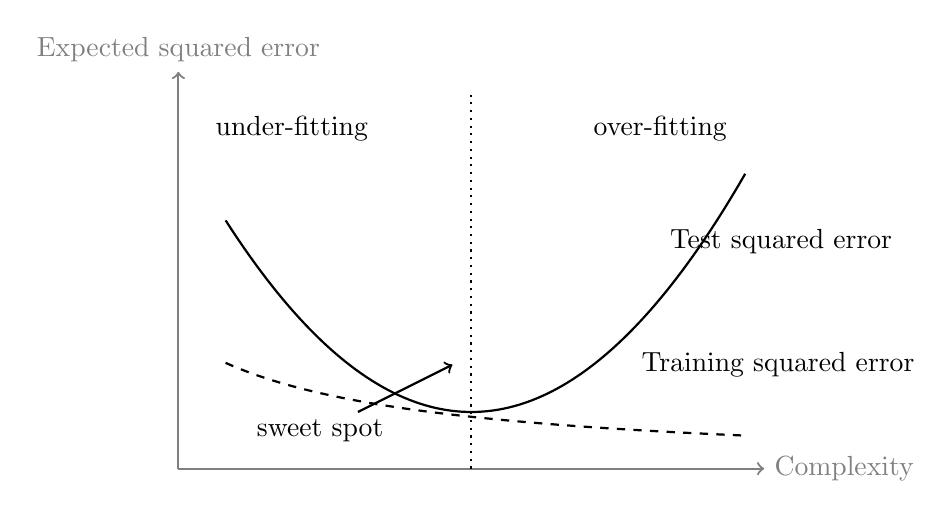
\begin{tikzpicture}[scale=1.2]
		% Axes
		\draw[->, thick, gray] (0,0) -- (6.2,0) node[right] {Complexity};
		\draw[->, thick, gray] (0,0) -- (0,4.2) node[above] {Expected squared error};
		
		% Labels for under-fitting and over-fitting
		\node at (1.2,3.6) {under-fitting};
		\node at (5.1,3.6) {over-fitting};
		
		% Training risk curve
		\draw[thick, dashed, domain=0.5:6, samples=100] plot(\x, {1.4/(0.5*\x + 1)});
		\node[right] at (4.8,1.1) {Training squared error};
		
		% Test risk curve
		\draw[thick, domain=0.5:6, samples=100] plot(\x, {0.3*(\x - 3.1)^2 + 0.6});
		\node[right] at (5.1,2.4) {Test squared error};
		
		% Sweet spot annotation
		\draw[->, thick] (1.9,0.6) -- (2.9,1.1);
		\node[align=center] at (1.5,0.4) {sweet spot};
		
		% Vertical line at optimal capacity
		\draw[dotted, thick] (3.1,0) -- (3.1,4);
		
	\end{tikzpicture}
\begin{tablenotes}
	\item \small{\textbf{Notes:} Curves for training squared error (dashed line) and test squared error (solid line). The classical U-shaped error curve arising from the bias–variance trade-off.}
\end{tablenotes}
\caption{\textit{Bias-variance trade-off} in machine learning.}
\label{fig:bias_var}
\end{figure}
    
To avoid overfitting in machine learning, an important step called \textit{cross-validation} is often employed. This involves splitting the dataset into multiple parts (called \textit{folds}) and systematically training and testing models on these parts \cite{hastie2009elements,efron2021computer}. The main goal is to evaluate how well models generalize to ``unseen data''.

There is a compelling justification for cross-validation within Bayesian inference proposed by \cite{Bernardo1994} in their section 6.1.6. The point of departure is to assume an $\mathcal{M}$-open view of nature, in which there exists a set of models $\mathcal{M} = \left\{M_j : j \in J\right\}$ under comparison, but none of them represents the true data-generating process, which is assumed to be unknown. Nevertheless, we can compare the models in $\mathcal{M}$ based on their posterior risk functions (see Chapter~\ref{chap1}) without requiring the specification of a true model. In this framework, we select the model that minimizes the posterior expected loss. Unfortunately, we cannot explicitly compute this posterior expected loss due to the lack of knowledge of the true posterior distribution under the $\mathcal{M}$-open assumption.\footnote{This is not the case under an $\mathcal{M}$-closed view of nature, where one of the candidate models is assumed to be the true data-generating process. In that setting, the posterior distribution becomes a mixture distribution with mixing probabilities given by the posterior model probabilities (see Chapter~\ref{chap10}).}

Given the expected loss conditional on model \( j \) for a predictive problem, where the action \( a \) is chosen to minimize the posterior expected loss:
\begin{align*}
	\mathbb{E}_{y_0}[L(Y_0,a) \mid M_j, \mathbf{y}] &= \int_{\mathcal{Y}_0} L(y_0, a \mid M_j, \mathbf{y}) \, \pi(y_0 \mid \mathbf{y}) \, dy_0,
\end{align*}
we note that there are \( N \) possible partitions of the dataset \( \mathbf{y} = \{y_1, y_2, \dots, y_N\} \) following a leave-one-out strategy, i.e., \( \mathbf{y} = \{\mathbf{y}_{-k}, y_k\} \), for \( k = 1, \dots, N \), where \( \mathbf{y}_{-k} \) denotes the dataset excluding observation \( y_k \). Assuming that \( \mathbf{y} \) is exchangeable, meaning its joint distribution is invariant to reordering, and that \( N \) is large, then \( \mathbf{y}_{-k} \) and \( y_k \) are good proxies for \( \mathbf{y} \) and \( y_0 \), respectively. Consequently,
\begin{align*}
	\frac{1}{K} \sum_{k=1}^K L(y_k, a \mid M_j, \mathbf{y}_{-k}) 
	\stackrel{p}{\rightarrow}\int_{\mathcal{Y}_0} L(y_0, a \mid M_j, \mathbf{y}) \, \pi(y_0 \mid \mathbf{y}) \, dy_0,
\end{align*}
by the law of large numbers, as \( N \to \infty \) and \( K \to \infty \).

Thus, we can select a model by minimizing the expected squared error based on its expected predictions \( \mathbb{E}[y_k \mid M_j, \mathbf{y}_{-k}] \); that is, we select the model with the lowest value of
\[
\frac{1}{K} \sum_{k=1}^K \left( \mathbb{E}[y_k \mid M_j, \mathbf{y}_{-k}] - y_k \right)^2.
\]

Note that if we want to compare two models based on their relative predictive accuracy using the log-score function \cite{martin2022optimal}, we select model \( j \) if
\begin{align*}
	\int_{\mathcal{Y}_0} \log\frac{p(y_0 \mid M_j, \mathbf{y})}{p(y_0 \mid M_l, \mathbf{y})} \, \pi(y_0 \mid \mathbf{y}) \, dy_0 > 0.
\end{align*}
However, we know that
\begin{align*}
	\frac{1}{K}\sum_{k=1}^K\log\frac{p(y_k \mid M_j, \mathbf{y}_{-k})}{p(y_k \mid M_l, \mathbf{y}_{-k})} 
	\stackrel{p}{\rightarrow} \int_{\mathcal{Y}_0} \log\frac{p(y_0 \mid M_j, \mathbf{y})}{p(y_0 \mid M_l, \mathbf{y})} \, \pi(y_0 \mid \mathbf{y}) \, dy_0,
\end{align*}
by the law of large numbers as \( N \to \infty \) and \( K \to \infty \).

This implies that we select model \( j \) over model \( l \) if
\begin{align*}
	\prod_{k=1}^K \left( \frac{p(y_k \mid M_j, \mathbf{y}_{-k})}{p(y_k \mid M_l, \mathbf{y}_{-k})} \right)^{1/K} 
	= \prod_{k=1}^K \left( B_{jl}(y_k, \mathbf{y}_{-k}) \right)^{1/K} > 1,
\end{align*}
where \( B_{jl}(y_k, \mathbf{y}_{-k}) \) is the Bayes factor comparing model \( j \) to model \( l \), based on the posterior \( \pi(\boldsymbol{\theta}_m \mid M_m, \mathbf{y}_{-k}) \) and the predictive \( \pi(y_k \mid \boldsymbol{\theta}_m) \), for \( m \in \{j, l\} \).

Thus, under the log-score function, cross-validation reduces to the geometric average of Bayes factors that evaluate predictive performance based on the leave-one-out samples \( \mathbf{y}_{-k} \).

\section{Regularization}\label{sec13_2}

In this century, the amount of available data continues to grow. This means we have access to more covariates for prediction, and we can also generate additional inputs to enhance the predictive power of our models. As a result, we often encounter \textit{wide} datasets, where the number of inputs may exceed the number of observations. Even in modest settings, we might have hundreds of inputs, and we can use them to identify which ones contribute to accurate predictions. However, we generally avoid using all inputs at once due to the risk of overfitting. Thus, we require a class of input selection or \textit{regularization}.

In the standard linear regression setting,
\begin{align*}
	\mathbf{y} &= \mathbf{1}_N \beta_0 + \mathbf{W}\boldsymbol{\beta} + \boldsymbol{\mu},
\end{align*}
where \(\mathbf{1}_N\) is an \(N\)-dimensional vector of ones, \(\mathbf{W}\) is the \(N \times K\) design matrix of inputs, and \(\boldsymbol{\mu} \sim \mathcal{N}(\mathbf{0}, \sigma^2 \mathbf{I}_N)\), there has been extensive development of techniques aimed at regularization within the Frequentist inferential framework. These include methods such as Ridge regression \cite{hoerl1970ridge}; discrete subset selection techniques like best subset selection \cite{furnival1974regressions}, forward selection, and backward stepwise selection \cite{hastie2009elements}; as well as continuous subset selection approaches such as the LASSO \cite{tibshirani1996regression}, the elastic net \cite{zou2005regularization}, and OSCAR \cite{bondell2008simultaneous}.

It is important to note, however, that Ridge regression does not perform variable selection; rather, it shrinks coefficient estimates toward zero without setting them exactly to zero.

Ridge regression and the LASSO can be viewed as special cases of a more general class of estimators known as \textit{Bridge regression} \cite{fu1998penalized}, which also admits a Bayesian interpretation. Consider the following penalized least squares criterion in the linear regression setting:
\begin{align*}
	\hat{\boldsymbol{\beta}}^{\text{Bridge}} = \arg\min_{\boldsymbol{\beta}} \left\{ \sum_{i=1}^N \left( y_i - \beta_0 - \sum_{k=1}^K \tilde{w}_{ik} \beta_k \right)^2 + \lambda \sum_{k=1}^K |\beta_k|^q \right\}, \quad q \geq 0,
\end{align*}
where \(\tilde{w}_{ik}\) denotes the standardized inputs. Standardizing inputs is important in variable selection problems to avoid issues caused by differences in scale; otherwise, variables with larger magnitudes will be penalized less and disproportionately influence the regularization path.

Interpreting \( |\beta_k|^q \) as proportional to the negative log-prior density of \( \beta_k \), the penalty shapes the contours of the prior distribution on the parameters. Specifically:
\begin{itemize}
	\item \( q = 0 \) corresponds to best subset selection, where the penalty counts the number of nonzero coefficients.
	\item \( q = 1 \) yields the LASSO, which corresponds to a Laplace (double-exponential) prior.
	\item \( q = 2 \) yields ridge regression, which corresponds to a Gaussian prior.  
	 
\end{itemize}

In this light, best subset selection, the LASSO, and ridge regression can be viewed as maximum a posteriori (MAP) estimators under different priors centered at zero \cite{Park2008}. However, they are not Bayes estimators in the strict sense, since Bayes estimators are typically defined as the posterior \textit{mean}. While ridge regression coincides with the posterior mean under a Gaussian prior \cite{Ishwaran2005}, the LASSO and best subset selection yield posterior modes.

This distinction is important because the Bayesian framework naturally incorporates regularization through the use of proper priors, which helps mitigate overfitting. Specifically, when proper shrinkage priors are used, the posterior balances data likelihood and prior information, thus controlling model complexity.

Furthermore, empirical Bayes methods, where the marginal likelihood is optimized, or cross-validation can be used to estimate the scale parameter of the prior covariance matrix for the regression coefficients. This scale parameter, in turn, determines the strength of regularization in ridge regression.

Note that regularization introduces bias into the parameter estimates because it constrains the model, shrinking the location parameters toward zero. However, it substantially reduces variance, as the estimates are prevented from varying excessively across samples. As a result, the mean squared error (MSE) of the estimates, which equals the sum of the squared bias and the variance, is often lower for regularization methods compared to ordinary least squares (OLS), which remains unbiased under the classical assumptions. This trade-off is particularly important when the goal is to identify causal effects, where unbiasedness may be preferred over predictive accuracy (see Chapter \ref{chap12}).

\subsection{Bayesian LASSO}\label{sec13_21}
Given the popularity of the LASSO as a variable selection technique, we present its Bayesian formulation in this subsection \cite{Park2008}. The Gibbs sampler for the Bayesian LASSO exploits the representation of the Laplace distribution as a scale mixture of normals. This leads to the following hierarchical representation of the model:
\begin{align*}
	\mathbf{y} \mid \beta_0, \boldsymbol{\beta}, \sigma^2, \mathbf{W} &\sim {N}(\mathbf{1}_N \beta_0 + \mathbf{W} \boldsymbol{\beta}, \sigma^2 \mathbf{I}_N), \\
	\boldsymbol{\beta} \mid \sigma^2, \tau_1^2, \dots, \tau_K^2 &\sim {N}(\mathbf{0}_K, \sigma^2 \mathbf{D}_{\tau}), \\
	\tau_1^2, \dots, \tau_K^2 &\sim \prod_{k=1}^K \frac{\lambda^2}{2} \exp\left\{ -\frac{\lambda^2}{2} \tau_k^2 \right\}, \\
	\sigma^2 &\sim \frac{1}{\sigma^2},\\
	\beta_0&\sim c,
\end{align*}
where $\mathbf{D}_{\tau} = \operatorname{diag}(\tau_1^2, \dots, \tau_K^2)$ and $c$ is a constant. 

After integrating out \( \tau_1^2, \dots, \tau_K^2 \), the conditional prior of \( \boldsymbol{\beta} \mid \sigma^2 \) is:
\begin{align*}
	\pi(\boldsymbol{\beta} \mid \sigma^2) &= \prod_{k=1}^K \frac{\lambda}{2 \sqrt{\sigma^2}} \exp\left\{ -\frac{\lambda}{\sqrt{\sigma^2}} |\beta_k| \right\},
\end{align*}
which implies that the log-prior is proportional to \( \lambda \sum_{k=1}^K |\beta_k| \), matching the penalty term in the LASSO optimization problem.

The conditional posterior distributions for the Gibbs sampler are \cite{Park2008}:
\begin{align*}
	\boldsymbol{\beta} \mid \sigma^2, \tau_1^2, \dots, \tau_K^2, \tilde{\mathbf{W}}, \tilde{\mathbf{y}} &\sim {N}(\boldsymbol{\beta}_n, \sigma^2 \mathbf{B}_n), \\
	\sigma^2 \mid \boldsymbol{\beta}, \tau_1^2, \dots, \tau_K^2, \tilde{\mathbf{W}}, \tilde{\mathbf{y}} &\sim \text{Inverse-Gamma}(\alpha_n/2, \delta_n/2), \\
	1/\tau_k^2 \mid \boldsymbol{\beta}, \sigma^2 &\sim \text{Inverse-Gaussian}(\mu_{kn}, \lambda_n),\\
	\beta_0\mid \sigma^2, \tilde{\mathbf{W}}, \tilde{\mathbf{y}} &\sim N(\bar{y},\sigma^2/N) 
\end{align*}
where:
\begin{align*}
	\boldsymbol{\beta}_n &= \mathbf{B}_n \tilde{\mathbf{W}}^{\top} \tilde{\mathbf{y}}, \\
	\mathbf{B}_n &= \left( \tilde{\mathbf{W}}^{\top} \tilde{\mathbf{W}} + \mathbf{D}_{\tau}^{-1} \right)^{-1}, \\
	\alpha_n &= (N - 1) + K, \\
	\delta_n &= (\tilde{\mathbf{y}} - \tilde{\mathbf{W}} \boldsymbol{\beta})^{\top} (\tilde{\mathbf{y}} - \tilde{\mathbf{W}} \boldsymbol{\beta}) + \boldsymbol{\beta}^{\top} \mathbf{D}_{\tau}^{-1} \boldsymbol{\beta}, \\
	\mu_{kn} &= \sqrt{ \frac{ \lambda^2 \sigma^2 }{ \beta_k^2 } }, \\
	\lambda_n &= \lambda^2,
\end{align*}
where $\tilde{\mathbf{W}}$ is the matrix of standardized inputs and $\tilde{\mathbf{y}}$ is the centered response vector.

Note that the posterior distribution of $\boldsymbol{\tau}$ depends on the data through $\boldsymbol{\beta}$ and $\sigma^2$, which is a typical feature of hierarchical models. In this formulation, we can interpret \( \tau_k \) as local shrinkage parameters, while \( \lambda \) acts as a global shrinkage parameter. Higher values of \( \tau_k \) and \( \lambda \) imply stronger shrinkage toward zero. \cite{Park2008} propose two approaches for specifying the global shrinkage parameter: empirical Bayes estimation or a fully Bayesian hierarchical specification, where \( \lambda^2 \) is assigned a Gamma prior.

We should acknowledge that the Bayesian LASSO is more computationally expensive than the Frequentist LASSO. However, it provides credible intervals for the parameters automatically. In contrast, obtaining standard errors in the Frequentist LASSO is more challenging, particularly for parameters estimated to be exactly zero \cite{kyung2010penalized}.\\

\textbf{Example: Simulation exercise to study the Bayesian LASSO performance}

We simulate the process \( y_i = \beta_0 + \sum_{k=1}^{10} \beta_k w_{ik}  + \mu_i \), where \( \beta_k \sim \mathcal{U}(-3, 3) \), \( \mu_i \sim \mathcal{N}(0, 1) \), and \( w_{ik} \sim \mathcal{N}(0, 1) \), $i=1,2,\dots,500$. Additionally, we generate 90 extra potential inputs from a standard normal distribution, which are included in the model specification. Our goal is to assess whether the Bayesian LASSO can successfully identify the truly relevant inputs.

We use the \textit{bayesreg} package in \textbf{R} to perform the Bayesian LASSO, using 5,000 MCMC draws and 1,000 burn-in iterations. The following code illustrates the simulation exercise and compares the posterior means with the true population values.

The summary of the fit and the plot comparing the population parameters with the posterior means show that the Bayesian LASSO is able to identify the variables that are relevant in the data generating process. In Exercise 1, we propose programming the Gibbs sampler from scratch, assuming a hierarchical structure for the global shrinkage parameter, and comparing the results with those obtained using the \textit{monomvn} package.

\begin{tcolorbox}[enhanced,width=4.67in,center upper,
	fontupper=\large\bfseries,drop shadow southwest,sharp corners]
	\textit{R code. The Bayesian LASSO}
	\begin{VF}
		\begin{lstlisting}[language=R]
rm(list = ls()); set.seed(10101)
library(bayesreg)
# Parameters
n <- 500  # sample size
p <- 100  # number of predictors
s <- 10   # number of non-zero coefficients
# Generate design matrix
X <- matrix(rnorm(n * p), nrow = n, ncol = p)
# True beta: first s coefficients are non-zero, rest are zero
beta_true <- c(runif(s, -3, 3), rep(0, p - s))
# Generate response with some noise
sigma <- 1
y <- X %*% beta_true + rnorm(n, sd = sigma)
df <- data.frame(X,y)
### Using bayesreg ###
# Fit the model
fit <- bayesreg::bayesreg(y ~ X, data = df, model = "gaussian", prior = "lasso", 
n.samples = 5000, burnin = 1000)
# Check summary
summary(fit)
# Extract posterior means of beta
beta_post_mean <- rowMeans(fit$beta)
# Compare true vs estimated
plot(beta_true, beta_post_mean, pch = 19, col = "steelblue",
xlab = "True beta", ylab = "Posterior mean of beta",
main = "Bayesian LASSO Shrinkage")
abline(0, 1, col = "red", lty = 2)
\end{lstlisting}
	\end{VF}
\end{tcolorbox}
  
\subsection{Stochastic search variable selection}\label{sec13_22}
Another well-known Bayesian strategy for variable selection in the presence of a large set of regressors (inputs) is \textit{stochastic search variable selection} (SSVS) \cite{george1993variable,George1997}. SSVS is a particular case of the broader class of \textit{spike-and-slab} priors, in which the prior distribution for the location parameters is specified as a hierarchical mixture that captures the uncertainty inherent in variable selection problems \cite{Ishwaran2005}. The hierarchical structure of the model is given by
\begin{align*}
	\mathbf{y} \mid \beta_0, \boldsymbol{\beta}, \sigma^2, \mathbf{W} &\sim {N}(\mathbf{1}_N \beta_0  + \mathbf{W} \boldsymbol{\beta}, \sigma^2 \mathbf{I}_N), \\
	\boldsymbol{\beta} \mid \sigma^2, \boldsymbol{\gamma} &\sim {N}(\mathbf{0}_K, \sigma^2 \mathbf{D}_{\gamma} \mathbf{R} \mathbf{D}_{\gamma}), \\
	\sigma^2 &\sim \text{Inverse-Gamma}\left(\frac{v}{2}, \frac{v\lambda_{\gamma}}{2}\right), \\
	\gamma_k &\sim \text{Bernoulli}(p_k),
\end{align*}
where \(p_k\) is the prior inclusion probability of regressor \(w_k\), that is, \(P(\gamma_k = 1) = 1 - P(\gamma_k = 0) = p_k\), \(\mathbf{R}\) is a correlation matrix, and \(\mathbf{D}_{\gamma}\) is a diagonal matrix whose \(kk\)-th element is defined as
\begin{align*}
	(\mathbf{D}_{\gamma})_{kk} &= 
	\begin{Bmatrix}
		v_{0k}, & \text{if } \gamma_k = 0, \\
		v_{1k}, & \text{if } \gamma_k = 1
	\end{Bmatrix}.
\end{align*}

This formulation implies that \(\beta_k \sim (1 - \gamma_k) {N}(0, v_{0k}) + \gamma_k {N}(0, v_{1k})\), where \(v_{0k}\) and \(v_{1k}\) are chosen such that \(v_{0k}\) is small and \(v_{1k}\) is large. Therefore, when the data favors \(\gamma_k = 0\) over \(\gamma_k = 1\), the corresponding \(\beta_k\) is shrunk toward zero, effectively excluding input \(k\) from the model. In this sense, \({N}(0, v_{0k})\) is a spike prior concentrated at zero, while \({N}(0, v_{1k})\) is a diffuse slab prior. A critical aspect of SSVS is the choice of the hyperparameters \(v_{0k}\) and \(v_{1k}\), as they determine the amount of shrinkage applied to the regression coefficients (see \cite{george1993variable,George1997} for details).

The assumption \(\gamma_k \sim \text{Bernoulli}(p_k)\) implies that the prior on the inclusion indicators is given by \(\pi(\boldsymbol{\gamma}) = \prod_{k=1}^K p_k^{\gamma_k} (1 - p_k)^{1 - \gamma_k}\). This means that the inclusion of input \(k\) is independent of the inclusion of any other input \(j \neq k\). A common choice is the uniform prior \(\pi(\boldsymbol{\gamma}) = 2^{-K}\), which corresponds to setting \(p_k = 1/2\), giving each regressor an equal chance of being included \cite{Ishwaran2005}.

A practical choice for the correlation matrix is to set \(\mathbf{R} \propto (\tilde{\mathbf{W}}^{\top} \tilde{\mathbf{W}})^{-1}\) \cite{george1993variable}. Regarding the hyperparameters \(v\) and \(\lambda_{\gamma}\), it is helpful to interpret \(\lambda_{\gamma}\) as a prior estimate of \(\sigma^2\), and \(v\) as the prior sample size associated with this estimate. In the absence of prior information, \cite{george1997approaches} recommend setting \(\lambda_{\gamma}\) equal to the least squares estimate of the variance from the \textit{saturated model}, that is, the model including all regressors, and \(v\) a small number, for instance, 0.01.

The conditional posterior distributions for the Gibbs sampler are \cite{george1993variable}:
\begin{align*}
	\boldsymbol{\beta} \mid \sigma^2, \gamma_1, \dots, \gamma_K, \tilde{\mathbf{W}}, \tilde{\mathbf{y}} &\sim {N}(\boldsymbol{\beta}_n, \mathbf{B}_n), \\
	\sigma^2 \mid \boldsymbol{\beta}, \gamma_1, \dots, \gamma_K, \tilde{\mathbf{W}}, \tilde{\mathbf{y}} &\sim \text{Inverse-Gamma}(\alpha_n/2, \delta_n/2), \\
	\gamma_k \mid \boldsymbol{\beta}, \sigma^2 &\sim \text{Bernoulli}(p_{kn}),\\
\end{align*}
where:
\begin{align*}
	\boldsymbol{\beta}_n &= \sigma^{-2} \mathbf{B}_n \tilde{\mathbf{W}}^{\top} \tilde{\mathbf{y}}, \\
	\mathbf{B}_n &= \left(\sigma^{-2} \tilde{\mathbf{W}}^{\top} \tilde{\mathbf{W}} + \mathbf{D}_{\gamma}^{-1}\mathbf{R}^{-1}\mathbf{D}_{\gamma}^{-1} \right)^{-1}, \\
	\alpha_n &= N + v, \\
	\delta_n &= (\tilde{\mathbf{y}} - \tilde{\mathbf{W}} \boldsymbol{\beta})^{\top} (\tilde{\mathbf{y}} - \tilde{\mathbf{W}} \boldsymbol{\beta}) + v\lambda_{\gamma}, \\
	p_{kn} &= \frac{\pi(\boldsymbol{\beta}\mid \boldsymbol{\gamma}_{-k},\gamma_k=1)\times p_k}{\pi(\boldsymbol{\beta}\mid \boldsymbol{\gamma}_{-k},\gamma_k=1)\times p_k+\pi(\boldsymbol{\beta}\mid \boldsymbol{\gamma}_{-k},\gamma_k=0)\times (1-p_k)},
\end{align*}
where \(\tilde{\mathbf{W}}\) is the matrix of standardized inputs, \(\tilde{\mathbf{y}}\) is the centered response vector, \(\boldsymbol{\gamma}_{-k}\) denotes the vector composed of \(\gamma_1, \gamma_2, \dots, \gamma_K\) excluding \(\gamma_k\), and \(\pi(\boldsymbol{\beta} \mid \boldsymbol{\gamma}_{-k}, \gamma_k = \delta)\) is the posterior density of \(\boldsymbol{\beta}\) evaluated at \(\boldsymbol{\gamma}_{-k}\) and \(\gamma_k = \delta\), where \(\delta \in \{0,1\}\).

In general, it is wise to consider the inclusion of regressors jointly due to potential correlations among them; that is, the marginal frequency of \(\gamma_k = 1\) should be interpreted with caution. SSVS is more effective at identifying a good set of potential models rather than selecting a single best model.\\

\textbf{Example: Simulation exercise to study SSVS performance}

Let's use the simulation setting from the previous example to evaluate the performance of SSVS in uncovering the data-generating process. In particular, we use the \textit{BoomSpikeSlab} package to implement this example.

The analysis is performed using 5,000 posterior draws and the default prior. However, the package allows the user to modify the default prior via the \textit{SpikeSlabPrior} function.

The results show that the posterior inclusion probabilities for regressors 2 through 10 are 100\%, and the model with the highest posterior probability (94\%) includes all of these nine variables. However, the true data-generating process, which also includes regressor 1, receives a posterior model probability of 0\%. This is because the population coefficient of this regressor is essentially zero. The plot comparing the posterior means with the true population parameters indicates good performance of SSVS. In general, Bayesian methods for variable selection perform well, and the choice of the most suitable method largely depends on the prior specification \cite{ohara2009bayesian}.

\begin{tcolorbox}[enhanced,width=4.67in,center upper,
	fontupper=\large\bfseries,drop shadow southwest,sharp corners]
	\textit{R code. Stochastic search variable selection}
	\begin{VF}
		\begin{lstlisting}[language=R]
rm(list = ls()); set.seed(10101)
library(BoomSpikeSlab)
library(dplyr)
library(tibble)
# Parameters
n <- 500  # sample size
k <- 100  # number of predictors
s <- 10   # number of non-zero coefficients
# Generate design matrix
X <- matrix(rnorm(n * k), nrow = n, ncol = k)
# True beta: first s coefficients are non-zero, rest are zero
beta_true <- c(runif(s, -3, 3), rep(0, k - s))
# Generate response with some noise
sigma <- 1
y <- X %*% beta_true + rnorm(n, sd = sigma)
df <- data.frame(X,y)
### Using BoomSpikeSlab ###
#Scale regressors
W <- scale(X); yh <- y - mean(y)
prior <- SpikeSlabPrior(W, yh, 
expected.model.size = ncol(W)/2, # expect 50 nonzero predictors
prior.df = .01, # weaker prior than the default
prior.information.weight = .01,
diagonal.shrinkage = 0) # shrink to zero
niter <- 5000
######Estimate model########
SSBoomNew <- lm.spike(yh ~ W - 1, niter = niter, prior = prior)
Models <- SSBoomNew$beta != 0
PIP <- colMeans(SSBoomNew$beta != 0)
# Convert the logical matrix to a data frame and then to a tibble
df <- as.data.frame(Models); df_tbl <- as_tibble(df)
# Count identical rows
row_counts <- df_tbl %>% count(across(everything()), name = "frequency") %>% arrange(desc(frequency))
sum(row_counts[1:100,101])
# Ensure your vector and matrix are logical
trueModel <- c(rep(1, 10), rep(0, 90)) == 1  # convert to logical if needed
# Assume your matrix is named 'mat'
matching_rows <- apply(row_counts[,-101], 1, function(row) all(row == trueModel))
# Get indices (row numbers) where the match is TRUE
row_counts[which(matching_rows), 101]
# Coefficients
SummarySS <- summary(coda::mcmc(SSBoomNew$beta))
# Extract posterior means of beta
beta_post_mean <- SummarySS$statistics[, 1]
# Compare true vs estimated
plot(beta_true, beta_post_mean, pch = 19, col = "steelblue",
xlab = "True beta", ylab = "Posterior mean of beta",
main = "SSVS Shrinkage")
abline(0, 1, col = "red", lty = 2)
\end{lstlisting}
	\end{VF}
\end{tcolorbox}

The examples and exercises presented thus far have considered scenarios in which the number of inputs is smaller than the number of observations ($K < N$). In Exercise 4, we challenge the Bayesian LASSO and SSVS in a setting where the number of inputs exceeds the sample size ($K > N$). As you will observe in that experiment, both the Bayesian LASSO and SSVS perform well. However, the Bayesian LASSO requires more time to produce results compared to SSVS in this exercise. \cite{rockova2018spike} propose a connection between the LASSO and spike-and-slab priors for variable selection in linear models, offering oracle properties and optimal posterior concentration even in high-dimensional settings where $K > N$.

In addition, there are other Bayesian methods for regularization, such as the spike-and-slab approach proposed by \cite{Ishwaran2005} and non-local priors introduced by \cite{johnson2012bayesian}, which can be implemented using the \textbf{R} packages \textit{spikeslab} and \textit{mombf}, respectively.

%\subsection{Non-local priors}\label{sec13_23}

%\cite{johnson2012bayesian}: R package mombf link: https://cran.r-project.org/web/packages/mombf/index.html

\section{Bayesian additive regression trees}\label{sec13_3}

A Classification and Regression Tree (CART) is a method used to predict outcomes based on inputs without assuming a parametric model. It is referred to as a classification tree when the outcome variable is qualitative, and as a regression tree when the outcome variable is quantitative. The method works by recursively partitioning the dataset into smaller, more homogeneous subsets using decision rules based on the input variables. For regression tasks, CART selects splits that minimize prediction error, typically measured by the sum of squared residuals. For classification problems, it aims to create the purest possible groups, using criteria such as Gini impurity or entropy. The result is a tree-like structure in which each internal node represents a decision based on one variable, and each leaf node corresponds to a prediction. CART was popularized in the statistical community by \cite{breiman1984classification}.

Figure \ref{fig:tree} displays a binary regression tree with two variables: one continuous ($x_1$) and one categorical ($x_2 \in {A, B, C}$). The tree has seven nodes in total, four of which are terminal nodes ($B = 4$), dividing the input space $\mathbf{x} = (x_1, x_2)$ into four non-overlapping regions. Each internal node indicates the splitting variable and rule, while each terminal node shows the value $\theta_b$, representing the conditional mean of $y$ given $\mathbf{x}$.

The first split is based on the rule $x_1 \leq 5$ (left) versus $x_1 > 5$ (right). The leftmost terminal node corresponds to $x_2 \in {A}$ with $\mu_1 = 2$. The second terminal node, with $\mu_2 = 3$, is defined by $x_1 \leq 3$ and $x_2 \in {B, C}$. The third node assigns $\mu_3 = 5$ for $3 < x_1 \leq 5$ and $x_2 \in {B, C}$. Finally, the rightmost terminal node assigns $\mu_4 = 8$ for all observations with $x_1 > 5$.

\begin{figure}[h!]
	\centering
\begin{tikzpicture}[
	level distance=2.5cm,
	sibling distance=4cm,
	every node/.style={font=\small},
	ellipseNode/.style={draw, ellipse, minimum width=1.2cm, minimum height=0.7cm},
	rectNode/.style={draw, rectangle, minimum width=1.8cm, minimum height=0.9cm},
	edge from parent/.style={draw, -{Latex[length=2mm]}, line width=0.6pt},
	level 2/.style={sibling distance=3.2cm},
	level 3/.style={sibling distance=2.4cm}
	]
	
	% Root node
	\node[ellipseNode] (root) {}
	child { % Left subtree
		node[ellipseNode] (a1) {}
		child {
			node[rectNode] {$\mu_1 = 2$}
			edge from parent node[left] {$x_2 \in \{A\}$}
		}
		child {
			node[ellipseNode] (a2) {}
			child {
				node[rectNode] {$\mu_2 = 3$}
				edge from parent node[left] {$x_1 \leq 3$}
			}
			child {
				node[rectNode] {$\mu_3 = 5$}
				edge from parent node[right] {$x_1 > 3$}
			}
			edge from parent node[right] {$x_2 \in \{B,C\}$}
		}
		edge from parent node[left] {$x_1 \leq 5$}
	}
	child { % Right subtree
		node[rectNode] {$\mu_4 = 8$}
		edge from parent node[right] {$x_1 > 5$}
	};
	
\end{tikzpicture}
\begin{tablenotes}
	\item \small{\textbf{Notes:} Decision tree with one continuous variable ($x_1$) and one categorical variable ($x_2 \in \{A, B, C\}$). The tree has four terminal nodes, each associated with a value denoted by $\mu_b$.}
\end{tablenotes}
\caption{\textit{Decision tree}.}
\label{fig:tree}
\end{figure}	

We can view a CART model as specifying the conditional distribution of \( y \) given the vector of features \( \mathbf{x} = [x_1, x_2, \dots, x_K]^{\top} \). There are two main components: (i) the binary tree structure \( T \), which consists of a sequence of binary decision rules of the form \( x_k \in A \) versus \( x_k \notin A \), where \( A \) is a subset of the range of \( x_k \), and \( B \) terminal nodes that define a non-overlapping and exhaustive partition of the input space; and (ii) the parameter vector \( \boldsymbol{\theta} = [\mu_1, \mu_2, \dots, \mu_B]^{\top} \) and $\sigma^2$, where each \( \mu_b \) corresponds to the parameter associated with terminal node \( b \), and $\sigma^2$ is the variance. Consequently, the response \( y \mid \mathbf{x} \sim p(y \mid \mu_b,\sigma^2) \) if \( \mathbf{x} \) belongs to the region associated with terminal node \( b \), where \( p \) denotes a parametric distribution indexed by \( \mu_b \) and \( \sigma^2 \).

Assuming that \( y_{bi} \) is independently and identically distributed within each terminal node and independently across nodes, for \( b = 1, 2, \dots, B \) and \( i = 1, 2, \dots, n_b \), we have:
\begin{align*}
	p(\mathbf{y} \mid \mathbf{x}, T, \boldsymbol{\theta}, \sigma^2) &= \prod_{b=1}^B p(\mathbf{y}_b \mid \mu_b,\sigma^2) \\
	&= \prod_{b=1}^B \prod_{i=1}^{n_b} p(y_{bi} \mid \mu_b,\sigma^2),
\end{align*}
where $\mathbf{y}_b=[y_{b1}, y_{b2}, \dots, y_{bn_b}]^{\top}$ is the set of observations in the terminal node $b$.

\cite{chipman1998bayesian} introduced a Bayesian formulation of CART models, in which inference is carried out through a combination of prior specification on the binary tree structure \( T \) and the parameters \( \boldsymbol{\theta}, \sigma^2 \mid T \), along with a stochastic search strategy based on a Metropolis-Hastings algorithm. The transition kernels used in the algorithm include operations such as growing, pruning, changing, and swapping tree branches, and candidate trees are evaluated based on their marginal likelihood. This approach enables exploration of a richer set of potential tree models and offers a more flexible and effective alternative to the greedy algorithms commonly used in classical CART. 

While CART is a simple yet powerful tool, it is prone to overfitting. To mitigate this, ensemble methods such as boosting, bagging, and random forests are often used. \textit{Boosting} combines multiple weak trees sequentially, each correcting the errors of its predecessor, to create a strong predictive model \cite{freund1997decision}. \textit{Bagging} builds multiple models on bootstrapped datasets and averages their predictions to reduce variance \cite{breiman1996bagging}, and \textit{random forests} extend bagging by using decision trees and adding random input selection at each split to increase model diversity \cite{breiman2001random}. Although a single tree might overfit and generalize poorly, aggregating many randomized trees typically yields more accurate and stable predictions.

\cite{chipman2010bart} introduced Bayesian Additive Regression Trees (BART). The starting point is the model
\begin{align*}
	y_i &= f(\mathbf{x}_i) + \mu_i,
\end{align*}
where \( \mu_i \sim N(0, \sigma^2) \).

Thus, the conditional expectation \( \mathbb{E}[y_i \mid \mathbf{x}_i] = f(\mathbf{x}_i) \) is approximated as
\begin{align*}
	f(\mathbf{x}_i) & \approx h(\mathbf{x}_i) \nonumber \\
	&= \sum_{j=1}^J g_j(\mathbf{x}_i \mid T_j, \boldsymbol{\theta}_j),
\end{align*}
that is, \( f(\mathbf{x}_i) \) is approximated by the sum of \( J \) regression trees. Each tree is defined by a structure \( T_j \) and a corresponding set of terminal node parameters \( \boldsymbol{\theta}_j \), where \( g_j(\mathbf{x}_i \mid T_j, \boldsymbol{\theta}_j) \) denotes the function that assigns the value \( \mu_{bj} \in \boldsymbol{\theta}_j \) to \( \mathbf{x}_i \) according to the partition defined by \( T_j \).

The main idea is to construct this sum-of-trees model by imposing a prior that regularizes the fit, ensuring that the individual contribution of each tree remains small. Thus, each tree \( g_j \) explains a small and distinct portion of \( f \). This is achieved through Bayesian backfitting MCMC \cite{hastie2000bayesian}, where successive fits to the residuals are added. In this sense, BART can be viewed as a Bayesian version of boosting.

\cite{chipman2010bart} use the following prior structure
\begin{align*}
	\pi(\left\{(T_1,\boldsymbol{\theta}_1),(T_2,\boldsymbol{\theta}_2),\dots, (T_J,\boldsymbol{\theta}_J),\sigma^2\right\})&=\left[\prod_{j=1}^J\pi(T_j,\boldsymbol{\theta}_j)\right]\pi(\sigma)\\
	&=\left[\prod_{j=1}^J\pi(\boldsymbol{\theta}_j\mid T_j)\pi(T_j)\right]\pi(\sigma)\\
	&=\left[\prod_{j=1}^J\prod_{b=1}^B\pi(\mu_{bj}\mid T_j)\pi(T_j)\right]\pi(\sigma).
\end{align*}  

The prior for the binary tree structure has three components: (i) the probability that a node at depth \( d = 0, 1, \dots \) is nonterminal, given by \( \alpha(1 + d)^{-\beta} \), where \( \alpha \in (0,1) \) and \( \beta \in [0, \infty) \); the default values are \( \alpha = 0.95 \) and \( \beta = 2 \); (ii) a uniform prior over the set of available regressors to define the distribution of splitting variable assignments at each interior node; and (iii) a uniform prior over the discrete set of available splitting values to define the splitting rule assignment, conditional on the chosen splitting variable.

The prior for the terminal node parameters, \( \pi(\mu_{bj} \mid T_j) \), is specified as \( N(0, 0.5 / (k \sqrt{J})) \). The observed values of \( y \) are scaled and shifted to lie within the range \( y_{\text{min}} = -0.5 \) to \( y_{\text{max}} = 0.5 \), and the default value \( k = 2 \) ensures that  
\[
P_{\pi(\mu_{bj} \mid T_j)}\left(\mathbb{E}[y \mid \mathbf{x}] \in (-0.5, 0.5)\right) = 0.95.
\]
Note that this prior shrinks the effect of individual trees toward zero, ensuring that each tree contributes only a small amount to the overall prediction. Moreover, although the dependent variable is transformed, there is no need to transform the input variables, since the tree-splitting rules are invariant to monotonic transformations of the regressors.

The prior for \( \sigma^2 \) is specified as \( \pi(\sigma^2) \sim v\lambda / \chi^2_v \). \cite{chipman2010bart} recommend setting \( v = 3 \), and choosing \( \lambda \) such that \( P(\sigma < \hat{\sigma}) = q, q = 0.9 \), where \( \hat{\sigma} \) is an estimate of the residual standard deviation from a saturated linear model, i.e., a model including all available regressors when \( K < N \), or the standard deviation of \( y \) when \( K \geq N \). 

Finally, regarding the number of trees \( J \), the default value is 200. As \( J \) increases from 1, BART’s predictive performance typically improves substantially until it reaches a plateau, after which performance may degrade very slowly. However, if the primary goal is variable selection, using a smaller \( J \) is preferable, as it facilitates identifying the most important regressors by enhancing the internal competition among variables within a limited number of trees.

To sum up, the default hyperparameters are \( (\alpha, \beta, k, J, v, q) = (0.95, 2, 2, 200, 3, 0.9) \); however, cross-validation can be used to tune these hyperparameters if desired. BART's predictive performance appears to be relatively robust to the choice of hyperparameters, provided they are set to sensible values, except in cases where \( K > N \), in which cross-validated tuning tends to yield better performance, albeit at the cost of increased computational time.

Given this specification, we can use a Gibbs sampler that cycles through the \( J \) trees. At each iteration, we sample from the conditional posterior distribution
\[
\pi(T_j, \boldsymbol{\theta}_j \mid R_j, \sigma) = \pi(T_j \mid R_j, \sigma) \times \pi(\boldsymbol{\theta}_j \mid T_j, R_j, \sigma),
\]
where \( R_j = y - \sum_{k \neq j} g_k(\mathbf{x} \mid T_k, \boldsymbol{\theta}_k) \) represents the residuals excluding the contribution of the \( j \)-th tree.

The posterior distribution \( \pi(T_j \mid R_j, \sigma) \) is explored using a Metropolis-Hastings algorithm, where the candidate tree is generated by one of the following moves: (i) growing a terminal node with probability 0.25; (ii) pruning a pair of terminal nodes with probability 0.25; (iii) changing a nonterminal splitting rule with probability 0.4; or (iv) swapping a rule between a parent and child node with probability 0.1 \cite{chipman1998bayesian}.

The posterior distribution of \( \boldsymbol{\theta}_j \) is the product of the posterior distributions \( \pi(\mu_{jb} \mid T_j, R_j, \sigma) \), which are Gaussian. The posterior distribution of \( \sigma \) is inverse-gamma. The posterior draws of \( \mu_{bj} \) are then used to update the residuals \( R_{j+1} \), allowing the sampler to proceed to the next tree in the cycle. The number of iterations in the Gibbs sampler does not need to be very large; for instance, 200 burn-in iterations and 1,000 post-burn-in iterations typically work well.

As we obtain posterior draws from the sum-of-trees model, we can compute point estimates at each \( \mathbf{x}_i \) using the posterior mean, \( \mathbb{E}[y \mid \mathbf{x}_i] = f(\mathbf{x}_i) \). Additionally, pointwise measures of uncertainty can be derived from the quantiles of the posterior draws. We can also identify the most relevant predictors by tracking the relative frequency with which each regressor appears in the sum-of-trees model across iterations. Moreover, we can perform inference on functionals of \( f \), such as the \textit{partial dependence functions} \cite{friedman2001greedy}, which quantify the marginal effects of the regressors.

Specifically, if we are interested in the effect of \( \mathbf{x}_s \) on \( y \), while marginalizing over the remaining variables \( \mathbf{x}_c \), such that \( \mathbf{x} = [\mathbf{x}_s^{\top} \ \mathbf{x}_c^{\top}]^{\top} \), the partial dependence function is defined as
\begin{align*}
	f(\mathbf{x}_s) &= \frac{1}{N} \sum_{i=1}^N f(\mathbf{x}_s, \mathbf{x}_{ic}),
\end{align*}
where \( \mathbf{x}_{ic} \) denotes the \( i \)-th observed value of \( \mathbf{x}_c \) in the dataset.

Note that the calculation of the partial dependence function assumes that a subset of the variables is held fixed while averaging over the remainder. This assumption may be questionable when strong dependence exists among input variables, as fixing some variables while varying others may result in unrealistic or implausible combinations. Therefore, caution is warranted when interpreting the results.

\cite{linero2018bayesian} extended BART models to high-dimensional settings for prediction and variable selection, while \cite{hill2011bayesian, hahn2020bayesian} applied them to causal inference. The asymptotic properties of BART models have been studied by \cite{rockova2019on, rockova2020posterior, rockova2020semiparametric}.\\

\textbf{Example: Simulation exercise to study BART performance}

We use the \textit{BART} package \cite{sparapani2021nonparametric} in the \textbf{R} software environment to perform estimation, prediction, inference, and marginal analysis using Bayesian Additive Regression Trees. In addition to modeling continuous outcomes, this package also supports dichotomous, categorical, and time-to-event outcomes.

We adopt the simulation setting proposed by \cite{friedman1991multivariate}, which is also used by \cite{chipman2010bart}:
\begin{align*}
	y_i = 10\sin(\pi x_{i1}x_{i2}) + 20(x_{i3}-0.5)^2 + 10 x_{i4} + 5 x_{i5} + \mu_i,
\end{align*}
where \( \mu_i \sim N(0,1) \), for \( i = 1, 2, \dots, 500 \).

We set the hyperparameters to \( (\alpha, \beta, k, J, v, q) = (0.95, 2, 2, 200, 3, 0.9) \), with a burn-in of 100 iterations, a thinning parameter of 1, and 1,000 post-burn-in MCMC iterations. We analyze the trace plot of the posterior draws of \( \sigma \) to assess convergence, compare the true values of \( y \) with the posterior mean and 95\% predictive intervals for both the training and test sets (using 80\% of the data for training and 20\% for testing), and visualize the relative importance of the regressors across different values of \( J = 10, 20, 50, 100, 200 \).

\begin{tcolorbox}[enhanced,width=4.67in,center upper,
	fontupper=\large\bfseries,drop shadow southwest,sharp corners]
	\textit{R code. Bayesian additive regression trees}
	\begin{VF}
		\begin{lstlisting}[language=R]
rm(list = ls()); set.seed(10101)
library(BART); library(tidyr)
library(ggplot2); library(dplyr)
N <- 500; K <- 10
# Simulate the dataset
MeanFunct <- function(x){
	f <- 10*sin(pi*x[,1]*x[,2]) + 20*(x[,3]-.5)^2+10*x[,4]+5*x[,5]
	return(f)
}
sig2 <- 1
e <- rnorm(N, 0, sig2^0.5)
X <- matrix(runif(N*K),N,K)
y <- MeanFunct(X[,1:5]) + e
# Train and test
c <- 0.8
Ntrain <- floor(c * N)
Ntest <- N - Ntrain
X.train <- X[1:Ntrain, ]
y.train <- y[1:Ntrain]
X.test <- X[(Ntrain+1):N, ]
y.test <- y[(Ntrain+1):N]
# Hyperparameters
alpha <- 0.95; beta <- 2; k <- 2
v <- 3; q <- 0.9; J <- 200
# MCMC parameters
MCMCiter <- 1000; burnin <- 100; thinning <- 1
# Estimate BART
BARTfit <- wbart(x.train = X.train, y.train = y.train, x.test = X.test, base = alpha,
power = beta, k = k, sigdf = v, sigquant = q, ntree = J,
ndpost = MCMCiter, nskip = burnin, keepevery = thinning)

# Trace plot sigma
keep <- seq(burnin + 1, MCMCiter + burnin, thinning)
df_sigma <- data.frame(iteration = 1:length(keep), sigma = BARTfit$sigma[keep])
ggplot(df_sigma, aes(x = iteration, y = sigma)) + geom_line(color = "steelblue") + labs(title = "Trace Plot of Sigma", x = "Iteration", y = expression(sigma)) + theme_minimal()

# Prediction plot training
train_preds <- data.frame( y_true = y.train, mean = apply(BARTfit$yhat.train, 2, mean),
lower = apply(BARTfit$yhat.train, 2, quantile, 0.025), upper = apply(BARTfit$yhat.train, 2, quantile, 0.975)) %>% arrange(y_true) %>% mutate(index = row_number())
\end{lstlisting}
	\end{VF}
\end{tcolorbox}


\begin{tcolorbox}[enhanced,width=4.67in,center upper,
	fontupper=\large\bfseries,drop shadow southwest,sharp corners]
	\textit{R code. Bayesian additive regression trees}
	\begin{VF}
		\begin{lstlisting}[language=R]
ggplot(train_preds, aes(x = index)) + geom_ribbon(aes(ymin = lower, ymax = upper, fill = "95% Interval"), alpha = 0.4, show.legend = TRUE) + geom_line(aes(y = mean, color = "Predicted Mean")) + geom_line(aes(y = y_true, color = "True y")) + scale_color_manual(name = "Line", values = c("Predicted Mean" = "blue", "True y" = "black")) + scale_fill_manual(name = "Interval", values = c("95% Interval" = "lightblue")) + labs(title = "Training Data: Ordered Predictions with 95% Intervals",
x = "Ordered Index", y = "y") + theme_minimal()
# Prediction plot test
test_preds <- data.frame( y_true = y.test, mean = apply(BARTfit$yhat.test, 2, mean), lower = apply(BARTfit$yhat.test, 2, quantile, 0.025), upper = apply(BARTfit$yhat.test, 2, quantile, 0.975)) %>% arrange(y_true) %>% mutate(index = row_number())

ggplot(test_preds, aes(x = index)) + geom_ribbon(aes(ymin = lower, ymax = upper, fill = "95% Interval"), alpha = 0.4, show.legend = TRUE) + geom_line(aes(y = mean, color = "Predicted Mean")) + geom_line(aes(y = y_true, color = "True y")) + scale_color_manual(name = "Line", values = c("Predicted Mean" = "blue", "True y" = "black")) + scale_fill_manual(name = "Interval", values = c("95% Interval" = "lightblue")) + labs(title = "Test Data: Ordered Predictions with 95% Intervals",
x = "Ordered Index", y = "y") + theme_minimal()
# Relevant regressors
Js <- c(10, 20, 50, 100, 200)
VarImportance <- matrix(0, length(Js), K)
l <- 1
for (j in Js){
	BARTfit <- wbart(x.train = X.train, y.train = y.train, x.test = X.test, base = alpha,
	power = beta, k = k, sigdf = v, sigquant = q, ntree = j,
	ndpost = MCMCiter, nskip = burnin, keepevery = thinning)
	VarImportance[l, ] <- BARTfit[["varcount.mean"]]/j
	l <- l + 1
}

rownames(VarImportance) <- c("10", "20", "50", "100", "200")
colnames(VarImportance) <- as.character(1:10)
importance_df <- as.data.frame(VarImportance) %>% mutate(trees = rownames(.)) %>%
pivot_longer(cols = -trees, names_to = "variable", values_to = "percent_used")
importance_df$variable <- as.numeric(importance_df$variable)
importance_df$trees <- factor(importance_df$trees, levels = c("10", "20", "50", "100", "200"))

ggplot(importance_df, aes(x = variable, y = percent_used, color = trees, linetype = trees)) + geom_line() + geom_point() + scale_color_manual(values = c("10" = "red", "20" = "green", "50" = "blue", "100" = "cyan", "200" = "magenta")) + scale_x_continuous(breaks = 1:10) + labs(x = "variable", y = "percent used", color = "#trees", linetype = "#trees") + theme_minimal()
\end{lstlisting}
	\end{VF}
\end{tcolorbox}

Figure~\ref{figTraceplotsig} displays the trace plot of \(\sigma\), which appears to have reached a stationary distribution. However, the posterior draws are slightly lower than the true value (1).

\begin{figure}[!h]
	\centering
	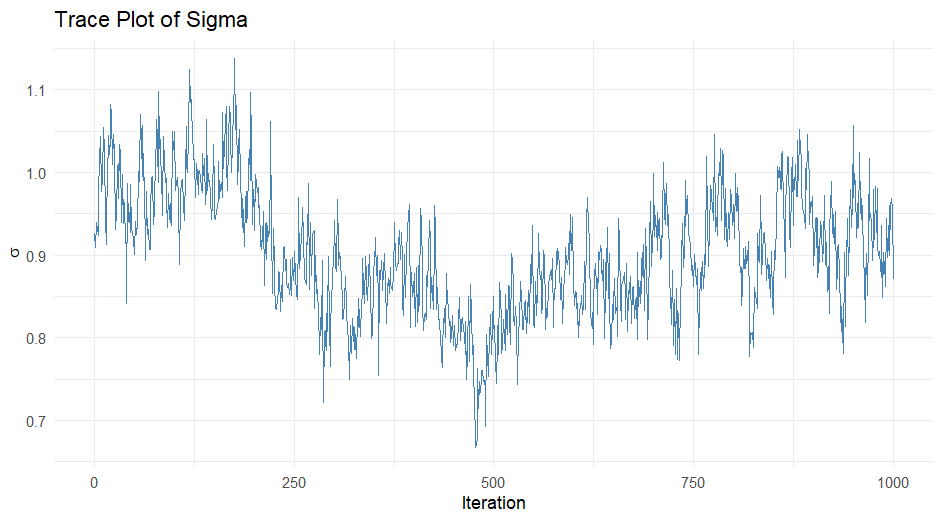
\includegraphics[width=340pt, height=200pt]{Chapters/chapter13/figures/Traceplotsig.png}
	\caption{Trace plot of the posterior draws of \(\sigma\) in the BART simulation.}
	\label{figTraceplotsig}
\end{figure}

Figures~\ref{figTrainingPred} and~\ref{figTestPred} compare the true values of \(y\) with the posterior mean and 95\% predictive intervals. The BART model performs well in both sets, and the intervals in the test set are notably wider than those in the training set.

\begin{figure}[!h]
	\centering
	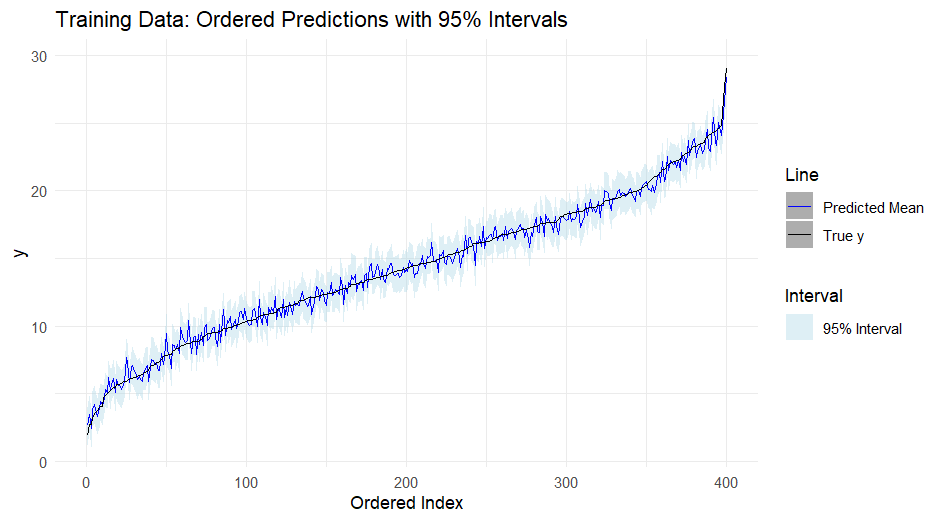
\includegraphics[width=340pt, height=200pt]{Chapters/chapter13/figures/TrainingPred.png}
	\caption{Training data: true \(y\) versus posterior mean and 95\% predictive intervals.}
	\label{figTrainingPred}
\end{figure}

\begin{figure}[!h]
	\centering
	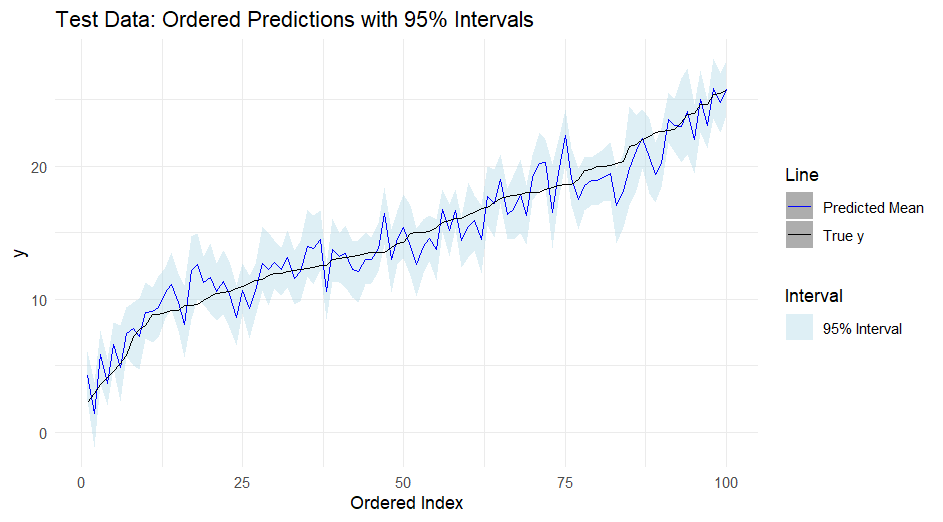
\includegraphics[width=340pt, height=200pt]{Chapters/chapter13/figures/TestPred.png}
	\caption{Test data: true \(y\) versus posterior mean and 95\% predictive intervals.}
	\label{figTestPred}
\end{figure}

Figure~\ref{figRelvVar} shows the relative frequency with which each variable is used in the trees, a measure of variable relevance. When the number of trees is small, the algorithm more clearly identifies the most relevant predictors (variables 1–5). As the number of trees increases, this discrimination gradually disappears.

\begin{figure}[!h]
	\centering
	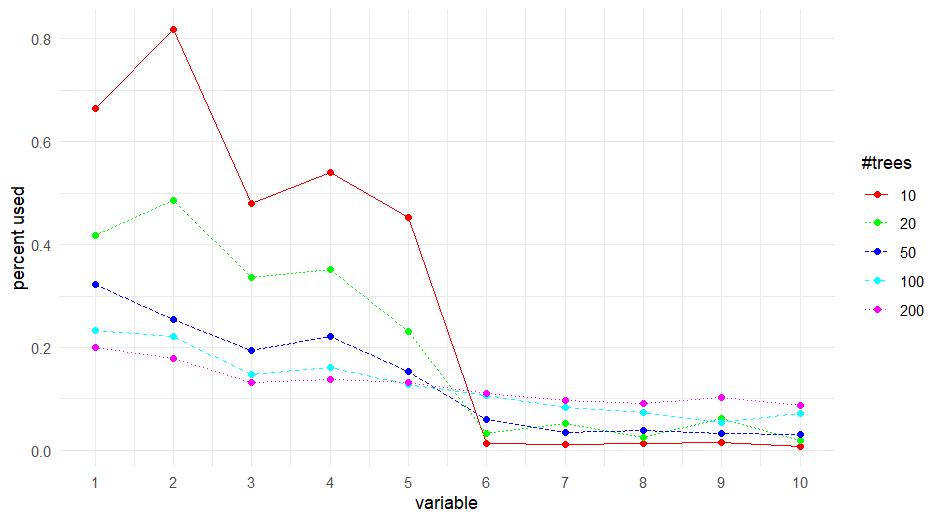
\includegraphics[width=340pt, height=200pt]{Chapters/chapter13/figures/RelvVar.png}
	\caption{Relative frequency of variable usage in the BART trees for different numbers of trees.}
	\label{figRelvVar}
\end{figure}

\section{Gaussian process}\label{13_4}
A Gaussian Process (GP) is an infinite collection of random variables, any finite subset of which follows a joint Gaussian distribution. A GP is fully specified by its mean function and covariance function, that is,
\begin{align*}
	f(\mathbf{x}) &\sim GP(m(\mathbf{x}), k(\mathbf{x}, \mathbf{x}')),
\end{align*}
where \( m(\mathbf{x}) = \mathbb{E}[f(\mathbf{x})] \) and \( k(\mathbf{x}, \mathbf{x}') = \mathbb{E}[(f(\mathbf{x}) - m(\mathbf{x}))(f(\mathbf{x}') - m(\mathbf{x}'))] \).  
It is common to assume \( m(\mathbf{x}) = 0 \) to simplify calculations, although this is not required.

Perhaps the most commonly used covariance function in Gaussian Processes (GPs) is the \textit{squared exponential} kernel (or \textit{radial basis function}) \cite{jacobi2024posterior}, defined as
\begin{align*}
	k(\mathbf{x}, \mathbf{x}') & = \sigma^2_f \exp\left(-\frac{1}{2l^2} \|\mathbf{x} - \mathbf{x}'\|^2\right),
\end{align*}
where \( \sigma^2_f \) is the signal variance, which controls the vertical variation (amplitude) of the function, \( l \) is the length-scale parameter, which determines how quickly the function varies with features distance, and \( \|\mathbf{x} - \mathbf{x}'\|^2 \) is the squared Euclidean distance between the feature vectors \( \mathbf{x} \) and \( \mathbf{x}' \).

The squared exponential kernel implies that the function is infinitely differentiable, leading to very smooth function draws. While this smoothness may be desirable in some applications, it can be too restrictive in others. Alternative kernels like the Matérn class allow for more flexibility by controlling the degree of differentiability \cite{rasmussen2006gaussian}.

A GP can be interpreted as a prior distribution over a space of functions. The starting point in working with GPs is the specification of this prior before any data are observed. The following code illustrates five sample paths drawn from a GP with a squared exponential kernel, assuming a signal variance \( \sigma_f^2 = 1 \) and a length-scale \( l = 0.2 \), evaluated over a grid of input values \( x \in [0,1] \). A small \textit{jitter term} is added to the covariance matrix to ensure numerical stability during simulation. Figure \ref{figGPsim} displays the five realizations drawn from the Gaussian Process.

\begin{tcolorbox}[enhanced,width=4.67in,center upper,
	fontupper=\large\bfseries,drop shadow southwest,sharp corners]
	\textit{R code. Simulation of five realizations: Gaussian process}
	\begin{VF}
		\begin{lstlisting}[language=R]
rm(list = ls())
set.seed(10101)

library(ggplot2); library(dplyr)
library(tidyr); library(MASS)

# Simulation setup
n <- 100
x <- seq(0, 1, length.out = n)
sigma_f <- 1
l <- 0.2
sigma_n <- 1e-8

# Squared Exponential Kernel function
SE_kernel <- function(x1, x2, sigma_f, l) {
	outer(x1, x2, function(a, b) sigma_f^2 * exp(-0.5 * (a - b)^2 / l^2))
}

K <- SE_kernel(x, x, sigma_f, l) + diag(sigma_n, n)
samples <- mvrnorm(n = 5, mu = rep(0, n), Sigma = K)

# Transpose and rename columns to f1, f2, ..., f5
samples_t <- t(samples)
colnames(samples_t) <- paste0("f", 1:5)

# Convert to tidy data frame
df <- data.frame(x = x, samples_t) |>
pivot_longer(cols = -x, names_to = "draw", values_to = "value")

# Plot
ggplot(df, aes(x = x, y = value, color = draw)) + geom_line(linewidth = 1) +
labs( title = "Simulated Gaussian Process Draws", x = "x", y = "f(x)", color = "Function" ) + theme_minimal(base_size = 14) + theme(legend.position = "top")
\end{lstlisting}
	\end{VF}
\end{tcolorbox}

\begin{figure}[!h]
	\centering
	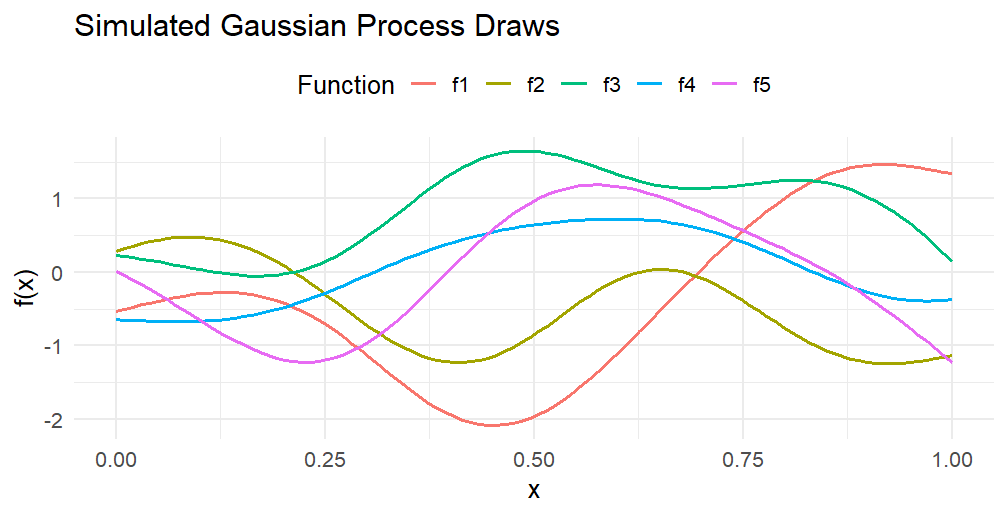
\includegraphics[width=340pt, height=200pt]{Chapters/chapter13/figures/GPsim.png}
	\caption{Simulation: Gaussian process.}
	\label{figGPsim}
\end{figure}

Thus, for any finite set of feature points \( \mathbf{x}_1, \mathbf{x}_2, \dots, \mathbf{x}_N \), the corresponding function values follow a multivariate Gaussian distribution:
\begin{align*}
	\mathbf{f} =
	\begin{bmatrix}
		f(\mathbf{x}_1) \\
		f(\mathbf{x}_2) \\
		\vdots \\
		f(\mathbf{x}_N)
	\end{bmatrix}
	\sim N(\mathbf{0}, \mathbf{K}(\mathbf{X}, \mathbf{X})),
\end{align*}
where the \( (i,j) \)-th entry of the covariance matrix \( \mathbf{K}(\mathbf{X}, \mathbf{X}) \) is given by \( \mathbf{K}_{ij} = k(\mathbf{x}_i, \mathbf{x}_j) \).

If we are interested in the properties of a function evaluated at a finite set of input points \( \{(f_i, x_i)\}_{i=1}^N\), inference can be performed using only those points, effectively disregarding the uncountably infinite values the function may take elsewhere.

The following code illustrates how to perform inference for a GP given four observed points \( \{(f_i, x_i)\}_{i=1}^4 \), assuming that the true underlying process is
\[
f_i = \sin(2\pi x_i).
\]
The inference is based on the properties of the conditional Gaussian distribution (see below). Figure~\ref{GPsimPoints} shows that the posterior mean (solid blue line) interpolates the observed points (red dots). Moreover, the level of uncertainty (light blue shaded area) increases in regions that are farther from the observed inputs, where the posterior mean tends to deviate more from the true underlying function (dashed green line).

In situations where the input locations can be selected—such as in experimental designs, \textit{active learning strategies} can be employed to choose the points that minimize predictive uncertainty. This is typically achieved by optimizing an \textit{acquisition function} that quantifies the expected informativeness of candidate locations \cite{settles2012active}. 

Consequently, GPs play a central role in \textit{Bayesian optimization}, a stochastic method for finding the maximum of expensive or unknown objective functions. In this approach, a prior is placed over the objective function, which is then updated using observed data to form a posterior distribution over possible functions. This posterior guides the selection of new input points by balancing exploration and exploitation through the acquisition function \cite{brochu2010tutorial}.

\begin{tcolorbox}[enhanced,width=4.67in,center upper,
	fontupper=\large\bfseries,drop shadow southwest,sharp corners]
	\textit{R code. Simulation: $f_i=\sin(2\pi x_i)$ and Gaussian process}
	\begin{VF}
		\begin{lstlisting}[language=R]
rm(list = ls()); set.seed(10101)
library(ggplot2); library(MASS)
# Define the squared exponential kernel
SE_kernel <- function(x1, x2, sigma_f, l) {
	outer(x1, x2, function(a, b) sigma_f^2 * exp(-0.5 * (a - b)^2 / l^2))
}
# Define the input space and observed points
x_star <- seq(0, 1, length.out = 200)
x0 <- c(0.1, 0.2, 0.5, 0.9)
y0 <- sin(2 * pi * x0)
# Hyperparameters
sigma_f <- 1
l <- 0.2
sigma_n <- 1e-8  # Jitter term for stability
# Compute covariance matrices
K_x0x0 <- SE_kernel(x0, x0, sigma_f, l) + diag(sigma_n, length(x0))
K_xstarx0 <- SE_kernel(x_star, x0, sigma_f, l)
K_xstarxstar <- SE_kernel(x_star, x_star, sigma_f, l) + diag(sigma_n, length(x_star))
# Compute posterior mean and covariance
K_inv <- solve(K_x0x0)
posterior_mean <- K_xstarx0 %*% K_inv %*% y0
posterior_cov <- K_xstarxstar - K_xstarx0 %*% K_inv %*% t(K_xstarx0)
# Sample from the posterior
sample_draw <- sin(2 * pi * x_star) 
# Compute 95% intervals
posterior_sd <- sqrt(diag(posterior_cov))
lower <- posterior_mean - 1.96 * posterior_sd
upper <- posterior_mean + 1.96 * posterior_sd
# Data frame for plotting
df <- data.frame(
x = x_star,
mean = posterior_mean,
lower = lower,
upper = upper,
sample = sample_draw
)
obs <- data.frame(x = x0, y = y0)
# Plot
ggplot(df, aes(x = x)) + geom_ribbon(aes(ymin = lower, ymax = upper), fill = "lightblue", alpha = 0.4) + geom_line(aes(y = mean), color = "blue", linewidth = 1.2) + geom_line(aes(y = sample), color = "darkgreen", linewidth = 1, linetype = "dashed") + geom_point(data = obs, aes(x = x, y = y), color = "red", size = 3) + labs( title = "Gaussian Process with Conditioning Points", x = "x", y = "f(x)", caption = "Blue: Posterior mean | Light blue: 95% interval | Dashed green: Population | Red: Observed points" ) + theme_minimal(base_size = 14)
\end{lstlisting}
	\end{VF}
\end{tcolorbox}

\begin{figure}[!h]
	\centering
	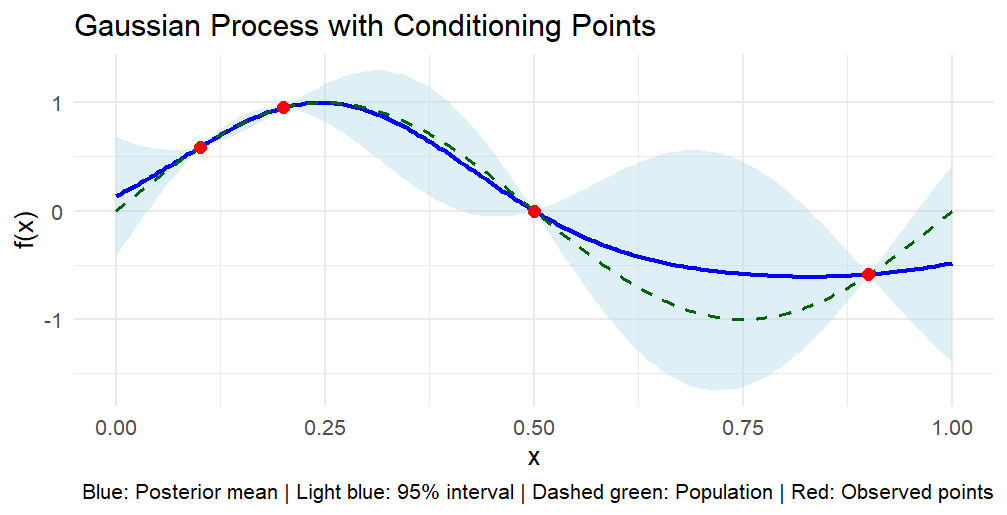
\includegraphics[width=340pt, height=200pt]{Chapters/chapter13/figures/GPsimPoints.png}
	\caption{Simulation: $f_i=\sin(2\pi x_i)$ and Gaussian process}
	\label{GPsimPoints}
\end{figure} 

In practice, we have an observed dataset \( \{(y_i, \mathbf{x}_i)\}_{i=1}^N \) such that
\begin{align*}
	y_i &= f(\mathbf{x}_i) + \mu_i,
\end{align*}
where \( \mu_i \overset{\text{i.i.d.}}{\sim} \mathcal{N}(0, \sigma^2) \). This means that $y_i$ is a noisy observation of $f(\mathbf{x}_i)$.

Thus, the marginal distribution of the observed outputs is
\[
\mathbf{y} \sim \mathcal{N}(\mathbf{0}, \mathbf{K}(\mathbf{X}, \mathbf{X}) + \sigma^2 \mathbf{I}_N),
\]
where \( \mathbf{K}(\mathbf{X}, \mathbf{X}) \) is the covariance matrix generated by the GP kernel evaluated at the training inputs.

Note that this implies the log marginal likelihood is given by
\begin{align*}
	\log p(\mathbf{y} \mid \mathbf{X}) &= -\frac{1}{2} \mathbf{y}^{\top} (\mathbf{K} + \sigma^2 \mathbf{I}_N)^{-1} \mathbf{y} - \frac{1}{2} \log \left| \mathbf{K} + \sigma^2 \mathbf{I}_N \right| - \frac{N}{2} \log 2\pi.
\end{align*}

We can adopt an empirical Bayes approach to estimate the hyperparameters of the GP prior by maximizing the log marginal likelihood with respect to the kernel parameters (e.g., \( \sigma_f^2 \), \( l \)) and the noise variance \( \sigma^2 \).

To make predictions at a new set of features \( \mathbf{X}_* \), we consider the joint distribution:
\begin{align*}
	\begin{bmatrix}
		\mathbf{y} \\
		\mathbf{f}_*
	\end{bmatrix}
	\sim \mathcal{N}\left(
	\mathbf{0},
	\begin{bmatrix}
		\mathbf{K}(\mathbf{X}, \mathbf{X}) + \sigma^2 \mathbf{I}_N & \mathbf{K}(\mathbf{X}, \mathbf{X}_*) \\
		\mathbf{K}(\mathbf{X}_*, \mathbf{X}) & \mathbf{K}(\mathbf{X}_*, \mathbf{X}_*)
	\end{bmatrix}
	\right).
\end{align*}

Using the conditional distribution of a multivariate Gaussian, the \textit{posterior predictive distribution} \cite{rasmussen2006gaussian} is:
\begin{align*}
	\mathbf{f}_* \mid \mathbf{y} &\sim \mathcal{N}(\bar{\mathbf{f}}_*, \operatorname{cov}(\mathbf{f}_*)),
\end{align*}
where
\begin{align*}
	\bar{\mathbf{f}}_* &= \mathbb{E}[\mathbf{f}_* \mid \mathbf{y}, \mathbf{X}, \mathbf{X}_*] = \mathbf{K}(\mathbf{X}_*, \mathbf{X}) [\mathbf{K}(\mathbf{X}, \mathbf{X}) + \sigma^2 \mathbf{I}_N]^{-1} \mathbf{y}, \\
	\operatorname{cov}(\mathbf{f}_*) &= \mathbf{K}(\mathbf{X}_*, \mathbf{X}_*) - \mathbf{K}(\mathbf{X}_*, \mathbf{X}) [\mathbf{K}(\mathbf{X}, \mathbf{X}) + \sigma^2 \mathbf{I}_N]^{-1} \mathbf{K}(\mathbf{X}, \mathbf{X}_*).
\end{align*}

Therefore, GP regression provides a flexible and efficient nonparametric framework for predicting unobserved responses, with accuracy that improves as more data become available. GPs are widely used due to their favorable computational properties, including the availability of closed-form expressions, and posterior consistency under mild conditions \cite{choi2007posterior, stuart2018posterior}. Moreover, predictive performance can be further enhanced by incorporating derivative information, as the derivative of a GP is itself a GP \cite{solak2003derivative,jacobi2024posterior}. 

However, a major limitation of GPs is the need to invert an \( N \times N \) covariance matrix, which requires \( O(N^3) \) computational operations, making them computationally expensive for large datasets. To address this, several scalable methods have been proposed that reduce the computational burden. For instance, \cite{wilson2015kernel,gardner2018product, pleiss2018constant} develop algorithms that reduce complexity to \( O(N) \).\\

\textbf{Example: Simulation exercise to study GP performance}

We simulate the process
\begin{align*}
	f_i & = \sin(2\pi x_{i1}) + \cos(2\pi x_{i2}) + \sin(x_{i1} x_{i2}),
\end{align*}
where $x_{i1}$ and $x_{i2}$ are independently drawn from a uniform distribution on the interval $[0, 1]$, for $i = 1, 2, \dots, 100$.

We use the \textit{DiceKriging} package in \textbf{R} to estimate and make predictions using a GP. This package applies maximum likelihood estimation to infer the length-scale parameters ($l_k$) and the signal variance ($\sigma_f^2$). Note that there are two separate length-scale parameters, one for each input variable. The following code illustrates how to carry out this example, and Figure~\ref{GPsim3D} displays a 3D plot with the observed points and the posterior mean surface. The package also provides pointwise credible intervals for the predictions.

\begin{tcolorbox}[enhanced,width=4.67in,center upper,
	fontupper=\large\bfseries,drop shadow southwest,sharp corners]
	\textit{R code. Simulation: $f_i=\sin(2\pi x_{i1}) + \cos(2\pi x_{i2}) + \sin(x_{i1} x_{i2})$ and Gaussian process}
	\begin{VF}
		\begin{lstlisting}[language=R]
# Load required packages
library(DiceKriging)
library(rgl)

# Simulate training data
set.seed(10101)
n_train <- 100
x1 <- runif(n_train)
x2 <- runif(n_train)
X_train <- data.frame(x1 = x1, x2 = x2)

# True function without noise
f_train <- sin(2 * pi * X_train$x1) + cos(2 * pi * X_train$x2) + sin(X_train$x1 * X_train$x2)

# Fit Gaussian Process
fit_km <- km(design = X_train, response = f_train, covtype = "gauss", nugget = 1e-10)

# Prediction grid
grid_points <- 30
x1_seq <- seq(0, 1, length.out = grid_points)
x2_seq <- seq(0, 1, length.out = grid_points)
grid <- expand.grid(x1 = x1_seq, x2 = x2_seq)

# Predict GP surface
pred <- predict(fit_km, newdata = grid, type = "UK")
z_pred <- matrix(pred$mean, nrow = grid_points, ncol = grid_points)

# Plot
persp3d(x = x1_seq, y = x2_seq, z = z_pred,
col = "lightblue", alpha = 0.7,
xlab = "x1", ylab = "x2", zlab = "GP Mean")
points3d(x = X_train$x1, y = X_train$x2, z = f_train, col = "red", size = 8)

fit_km@covariance@range.val # length-scale
fit_km@covariance@sd2 # Signal variance
\end{lstlisting}
	\end{VF}
\end{tcolorbox}

\begin{figure}[!h]
	\centering
	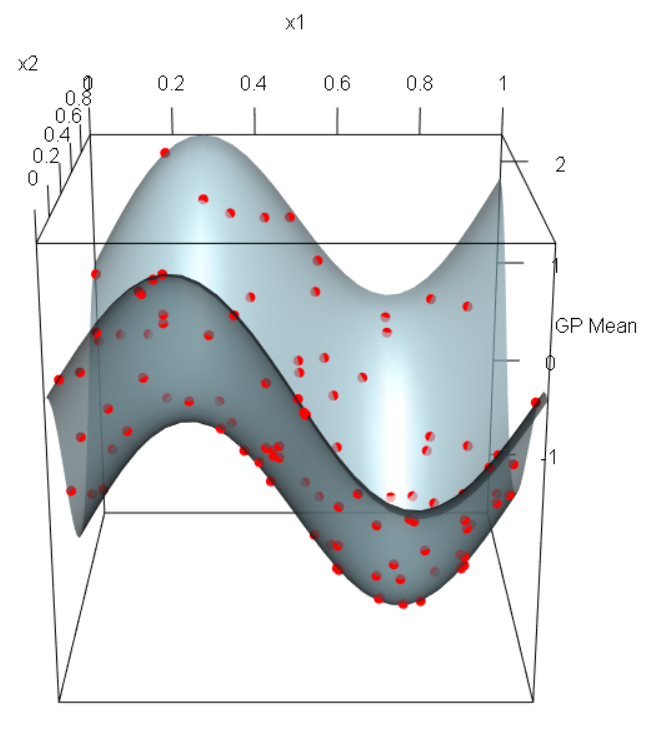
\includegraphics[width=340pt, height=200pt]{Chapters/chapter13/figures/GPsim3D.png}
	\caption{Simulation: $f_i=\sin(2\pi x_{i1}) + \cos(2\pi x_{i2}) + \sin(x_{i1} x_{i2})$ and Gaussian process}
	\label{GPsim3D}
\end{figure} 

A limitation of the \textit{DiceKriging} package is that it is designed for deterministic simulations and, consequently, does not estimate the noise variance. Therefore, in Exercise 7, we ask to simulate the process
\[
f_i = \sin(2\pi x_{i1}) + \cos(2\pi x_{i2}) + \sin(x_{i1} x_{i2}) + \mu_i,
\]
where \( \mu_i \overset{\text{i.i.d.}}{\sim} \mathcal{N}(0, 0.1^2) \), and to use an empirical Bayes approach to estimate the hyperparameters. These estimated hyperparameters should then be used to perform GP prediction.

\section{Tall data problems}\label{13_5}
In this section, we explore several methods developed to perform Bayesian inference when the sample size is large, particularly when there is a large number of observational units, commonly referred to as \textit{tall datasets}.

Bayesian inference in such settings is computationally demanding because each iteration of an MCMC algorithm requires evaluating the likelihood function over all \( N \) observations. For large \( N \), this renders standard MCMC methods prohibitively expensive. Recent efforts have focused on developing scalable Monte Carlo algorithms that significantly reduce the computational cost compared to standard approaches. One alternative is to use \textit{Variational Bayes} (see Chapter~\ref{chap15}); however, it can be challenging to implement and may exhibit limitations in uncertainty quantification, particularly for the joint posterior distribution. Another alternative is the \textit{Integrated Nested Laplace Approximation} (INLA, see Chapter~\ref{chap15}); however, its computational cost grows exponentially with the dimension of the parameter space. 

In scenarios where observations are assumed to be independent, two main frameworks have been proposed to scale MCMC algorithms: \textit{divide-and-conquer approaches} and \textit{subsampling-based algorithms}. Divide-and-conquer methods partition the dataset into disjoint subsets, run MCMC independently on each batch to obtain subposteriors, and then combine them to approximate the full posterior distribution. Subsampling-based algorithms, on the other hand, aim to reduce the number of data points used to evaluate the likelihood at each iteration, often relying on \textit{pseudo-marginal} MCMC methods \cite{andrieu2009pseudoefficient}. The key idea of pseudo-marginal MCMC is to augment the model with latent variables such that the sample average of the likelihood, computed over draws from these latent variables, provides an unbiased estimator of the marginal likelihood. This approach is particularly valuable when the marginal likelihood is not available in closed form. Moreover, the same principles can be adapted to reduce the computational burden of evaluating the log-likelihood. For an excellent review of divide-and-conquer and subsampling-based approaches, see \cite{bardenet2017markov}.

\subsection{Divide-and-conquer methods}
In \textit{divide-and-conquer} methods, the main idea is to partition the dataset and distribute the subsets across multiple computing machines/cores. An independent MCMC algorithm is then executed on each subset to obtain a corresponding \textit{subposterior} distribution. The central challenge lies in accurately and efficiently combining these subposteriors into a single approximation of the full posterior distribution. Several approaches have been proposed to address this issue. For instance, \cite{huang2005sampling,scott2016bayes, rendell2020global, scott2022bayes} introduce the \textit{Consensus Monte Carlo} algorithm; \cite{wang2013parallelizing} develop a method based on the \textit{Weierstrass sampler} for parallelizing MCMC; \cite{minsker2015scalable} propose using the \textit{geometric median of posterior distributions}; and \cite{wu2017average} suggest combining \textit{rescaled subposteriors}.

In divide-and-conquer methods, the dataset is partitioned into \( B \) disjoint batches \( \mathbf{y}_1, \mathbf{y}_2, \dots, \mathbf{y}_B \), and the posterior is rewritten using the identity:
\begin{align*}
	\pi(\boldsymbol{\theta} \mid \mathbf{y}) &\propto \prod_{b=1}^B \pi(\boldsymbol{\theta})^{1/B} p(\mathbf{y}_b \mid \boldsymbol{\theta}),
\end{align*}
which implies that the full posterior is proportional to the product of appropriately rescaled subposteriors.

\textit{Consensus Monte Carlo} (CMC) operates by running separate Monte Carlo algorithms on each subset in parallel, and then averaging the resulting posterior draws. Specifically, given samples \( \boldsymbol{\theta}_b^{(s)} \), for  \( b = 1, 2, \dots, B \) and \( s = 1, 2, \dots, S \), obtained independently from each batch \( \mathbf{y}_b \), the \( s \)-th draw from the consensus posterior is computed as:
\begin{align*}
	\boldsymbol{\theta}^{(s)} = \left( \sum_{b=1}^B \mathbf{w}_b \right)^{-1} \sum_{b=1}^B \mathbf{w}_b \boldsymbol{\theta}_b^{(s)},
\end{align*}
where the optimal weight is the inverse covariance matrix of the subposterior, i.e., \( \mathbf{w}_b = \operatorname{Var}^{-1}(\boldsymbol{\theta} \mid \mathbf{y}_b) \). In practice, one may use the marginal variances of each parameter to simplify the computation, which can still yield good performance.

When each subposterior \( \pi_b(\boldsymbol{\theta} \mid \mathbf{y}_b) \) is Gaussian, the full posterior \( \pi(\boldsymbol{\theta} \mid \mathbf{y}) \) is also Gaussian, and can be recovered exactly by combining the subposteriors using simple rules based on their means and covariances \cite{scott2016bayes, scott2022bayes}. In the non-Gaussian case, standard asymptotic results in Bayesian inference (see Chapter~\ref{chap1}) imply that the posterior distributions converge to a Gaussian distribution as the batch size increases. Alternative merging procedures that are more robust to non-Gaussianity have also been proposed \cite{neiswanger2013asymptotically, minsker2017robust}; however, it remains difficult to quantify the approximation error in these approaches. Moreover, this procedure is limited to continuous parameter spaces and may exhibit small-sample bias; that is, when the dataset is divided into small batches, the subposterior distributions may be biased. In such cases, jackknife bias corrections are recommended to reduce the overall approximation error.

In particular, we perform CMC following Algorithm~\ref{Alg:CMC} \cite{scott2016bayes}. Next, we compute the CMC posterior repeatedly, each time leaving out one of the \( B \) subsets. Let \( \pi_{-b}(\boldsymbol{\theta} \mid \mathbf{y}) \) denote the resulting posterior when subset \( b \) is excluded. The average of these leave-one-out posteriors is denoted by
\[
\bar{\pi}_{-b}(\boldsymbol{\theta} \mid \mathbf{y}) = \frac{1}{B} \sum_{b=1}^B \pi_{-b}(\boldsymbol{\theta} \mid \mathbf{y}).
\]
Then, the jackknife bias-corrected posterior is given by
\[
\pi_{\text{jk}}(\boldsymbol{\theta} \mid \mathbf{y}) = B \cdot \pi_{\text{CMC}}(\boldsymbol{\theta} \mid \mathbf{y}) - (B - 1) \cdot \bar{\pi}_{-b}(\boldsymbol{\theta} \mid \mathbf{y}),
\]
where \( \pi_{\text{CMC}}(\boldsymbol{\theta} \mid \mathbf{y}) \) is the original CMC posterior based on all \( B \) subsets.

\begin{algorithm}[h!]
	\caption{Consensus Monte Carlo algorithm}\label{Alg:CMC}
	\begin{algorithmic}[1]
		\State Divide the dataset into \( B \) disjoint batches $\mathbf{y}_1, \mathbf{y}_2, \dots, \mathbf{y}_B$
		\State Run $B$ separate MCMC algorithms to sample $\boldsymbol{\theta}_b^{(s)}\sim \pi(\boldsymbol{\theta}\mid \mathbf{y}_b)$, $b=1,2,\dots,B$, and $s=1,2,\dots,S$ using the prior distribution $\pi(\boldsymbol{\theta})^{1/B}$
		\State Combine the posterior draws using $\boldsymbol{\theta}^{(s)}=\left(\sum_{b=1}^B\mathbf{w}_b\right)^{-1} \sum_{b=1}^B\mathbf{w}_b \boldsymbol{\theta}^{(s)}_b$ using \( \mathbf{w}_b = \operatorname{Var}^{-1}(\boldsymbol{\theta} \mid \mathbf{y}_b) \)    		 			 
	\end{algorithmic} 
\end{algorithm}

The main difficulty is how to effectively merge the subposterior distributions, especially when their supports are not well-aligned. This misalignment can lead to poor scalability with an increasing number of batches. Moreover, most theoretical guarantees for these methods are asymptotic in the size of each batch, which may limit their performance in practice \cite{bardenet2017markov}.

\subsection{Subsampling-based algorithms}

An alternative to divide-and-conquer methods is to avoid evaluating the likelihood over all observations, which requires \( O(N) \) operations. Instead, the likelihood is approximated using a smaller subset of observations, \( n \ll N \), in order to reduce the computational burden of the algorithm. The starting point is the log-likelihood function for \( N \) independent observations:
\begin{align*}
	\log p(\mathbf{y} \mid \boldsymbol{\theta}) &= \sum_{i=1}^N \log p(y_i \mid \boldsymbol{\theta}).
\end{align*}
The literature has focused on the log-likelihood because it is a sum over independent contributions, which is analogous to the problem of estimating a population total.

A class of subsampling methods relies on estimating the marginal likelihood via the \textit{pseudo-marginal} approach. Examples include the confidence sampler \cite{bardenet2014towards}, the Firefly Monte Carlo algorithm \cite{Maclaurin2015}, whose relationship to subsampling MCMC is formally established in \cite{bardenet2017markov}, and approaches using data-expanded and parameter-expanded control variates \cite{quiroz2019speeding}.

The intuition behind the pseudo-marginal method is straightforward: introduce a set of auxiliary random variables \( \mathbf{z} \sim p(\mathbf{z}) \), such that the marginal likelihood can be written as an expectation with respect to \( \mathbf{z} \):
\[
\mathbb{E}_{\mathbf{z}}[p(\mathbf{y} \mid \boldsymbol{\theta}, \mathbf{z})] = \int_{\mathcal{Z}} p(\mathbf{y} \mid \boldsymbol{\theta}, \mathbf{z}) \, p(\mathbf{z}) \, d\mathbf{z} = p(\mathbf{y} \mid \boldsymbol{\theta}).
\]
This implies that
\[
\hat{p}(\mathbf{y} \mid \boldsymbol{\theta}) = \frac{1}{S} \sum_{s=1}^S p(\mathbf{y} \mid \boldsymbol{\theta}, \mathbf{z}^{(s)}),
\]
where \( \mathbf{z}^{(s)} \sim p(\mathbf{z}) \), is an unbiased estimator of the marginal likelihood.

As a result, the pseudo-marginal method enables exact simulation-based inference for \( p(\mathbf{y} \mid \boldsymbol{\theta}) \) in settings where the likelihood cannot be evaluated analytically \cite{andrieu2009pseudoefficient}, for instance, in non-linear random effects models (see also approximate methods such as \textit{approximate Bayesian computation} and \textit{Bayesian synthetic likelihood} in Chapter \ref{chap15}). \cite{andrieu2009pseudoefficient} show that replacing the likelihood with an unbiased and positive estimator within the Metropolis–Hastings (MH) algorithm yields samples from the correct posterior distribution.

The pseudo-marginal likelihood approach can also be applied in settings where the sample size is so large that evaluating the full likelihood at each iteration of an MCMC algorithm becomes computationally prohibitive. In such cases, the likelihood can be approximated using a small subset of observations, \( n \ll N \). The choice of the subset size \( n \) is particularly important, as it directly affects the variance of the likelihood estimator, which in turn is critical to ensuring an efficient Metropolis–Hastings (MH) algorithm.

In particular, a likelihood estimator with high variance may result in an accepted draw that overestimates the likelihood. As a consequence, subsequent proposals are unlikely to be accepted, causing the algorithm to become stuck and leading to a very low acceptance rate. Therefore, the choice of \( n \) determines the computational efficiency of the algorithm: a small \( n \) increases the estimator's variance, which reduces the acceptance rate, whereas a large \( n \) increases the number of likelihood evaluations per iteration.

\cite{quiroz2018subsampling} recommend targeting a likelihood estimator variance between 1 and 3.3 to optimize computational efficiency, as supported by the findings of \cite{pitt2012some}.

Let \( \ell_i(y_i \mid \boldsymbol{\theta}) = \log p(y_i \mid \boldsymbol{\theta}) \) denote the contribution of the \( i \)-th observation to the log-likelihood, and let \( z_1, \dots, z_N \) be latent binary variables such that \( z_i = 1 \) indicates that \( y_i \) is included in a subsample of size \( n \), selected without replacement. Then, an unbiased estimator of the log-likelihood is given by
\begin{align*}
	\hat{\ell}(\mathbf{y} \mid \boldsymbol{\theta}) & = \frac{N}{n} \sum_{i=1}^N \ell_i(y_i \mid \boldsymbol{\theta}) z_i.
\end{align*}

However, note that what we require is an unbiased estimator of the likelihood, not the log-likelihood. Consequently, a bias correction is needed:
\begin{align*}
	\hat{p}(\mathbf{y} \mid \boldsymbol{\theta}) & = \exp\left\{ \hat{\ell}(\mathbf{y} \mid \boldsymbol{\theta}) - \frac{1}{2} \sigma^2_{\hat{\ell}}(\boldsymbol{\theta}) \right\},
\end{align*}
where \( \sigma^2_{\hat{\ell}}(\boldsymbol{\theta}) \) denotes the variance of \( \hat{\ell}(\mathbf{y} \mid \boldsymbol{\theta}) \) \cite{ceperley1999penalty}. This correction is exact if \( \sigma^2_{\hat{\ell}}(\boldsymbol{\theta}) \) is known and \( \hat{\ell}(\mathbf{y} \mid \boldsymbol{\theta}) \) follows a normal distribution.

Given the importance of controlling the variance of the log-likelihood estimator in subsampling methods, and the limitations of simple random sampling in achieving low variability, \cite{quiroz2019speeding} propose a highly efficient, unbiased estimator of the log-likelihood based on \textit{control variates}, specifically through data-expanded and parameter-expanded control variates. 
The key idea is to construct a function \( q_i(\boldsymbol{\theta}) \) that is highly correlated with the log-likelihood contribution \( \ell_i(y_i \mid \boldsymbol{\theta}) \), thereby stabilizing the log-likelihood estimator. In particular, \cite{quiroz2019speeding} introduce a \textit{difference estimator} of the form:
\begin{align*}
	\hat{\ell}_{\mathrm{DE}}(\mathbf{y} \mid \boldsymbol{\theta}, \mathbf{z}) = \sum_{i=1}^N q_i(\boldsymbol{\theta}) + \frac{N}{n} \sum_{i: z_i = 1} \left( \ell_i(y_i \mid \boldsymbol{\theta}) - q_i(\boldsymbol{\theta}) \right).
\end{align*}
This estimator \( \hat{\ell}_{\mathrm{DE}}(\mathbf{y} \mid \boldsymbol{\theta}, \mathbf{z}) \) is unbiased for the full log-likelihood \( \log p(\mathbf{y} \mid \boldsymbol{\theta}) \).

\cite{quiroz2019speeding} propose constructing \( q_i(\boldsymbol{\theta}) \) using a second-order Taylor expansion of the log-likelihood around a central value of \( \boldsymbol{\theta} \), such as the mode. An alternative approach is to perform a second-order Taylor expansion around the nearest centroid of each observation, where the centroids are obtained from a pre-clustering of the data.

The first approach can perform poorly when the current draw \( \boldsymbol{\theta} \) is far from the central expansion point, leading to inaccurate approximations. The second approach encounters difficulties in high-dimensional settings due to the curse of dimensionality: many observations will be far from their assigned centroid. To address these issues, the authors propose an adaptive strategy: initialize the algorithm using data-expanded control variates, and switch to parameter-expanded control variates once the sampler reaches a region closer to the center of the parameter space.

It is important to note that this strategy targets an approximation to the posterior distribution, due to the small bias introduced by the difference estimator. However, this bias diminishes rapidly and has a negligible impact on the quality of the posterior inference.

Once a good estimator of the log-likelihood is obtained, meaning it has low variance, the likelihood can be recovered using the appropriate bias correction. This corrected likelihood estimator is then used within the acceptance probability of the Metropolis–Hastings algorithm (see Section \ref{sec512}), resulting in the so-called pseudo-marginal Metropolis–Hastings (PMMH) method. This strategy significantly reduces computational cost in tall data settings.

Another class of subsampling methods, which does not rely on the pseudo-marginal likelihood, consists of stochastic gradient MCMC algorithms. These methods begin based on ideas from stochastic gradient descent \cite{robbins1951stochastic} and the Langevin diffusion-based stochastic differential equations.

The point of departure is the unnormalized posterior distribution:
\begin{align*}
	\pi(\boldsymbol{\theta} \mid \mathbf{y}) &\propto \pi(\boldsymbol{\theta}) \prod_{i=1}^{N} p(y_i \mid \boldsymbol{\theta}) \\
	&= \exp\left\{ \sum_{i=1}^N \left[ \frac{1}{N} \log \pi(\boldsymbol{\theta}) + \log p(y_i \mid \boldsymbol{\theta}) \right] \right\} \\
	&= \exp\left\{ -\sum_{i=1}^N U_i(\boldsymbol{\theta}) \right\} \\
	&= \exp\left\{ -U(\boldsymbol{\theta}) \right\},
\end{align*}
where \( \boldsymbol{\theta} \in \mathbb{R}^K \), \( U_i(\boldsymbol{\theta}) = -\frac{1}{N} \log \pi(\boldsymbol{\theta}) - \log p(y_i \mid \boldsymbol{\theta}) \), and \( U(\boldsymbol{\theta}) = \sum_{i=1}^N U_i(\boldsymbol{\theta}) \) is assumed to be continuous and differentiable almost everywhere.  

The advantage of this formulation is that, under mild regularity conditions \cite{roberts1996exponential}, the Langevin diffusion process
\begin{align*}
	d\boldsymbol{\theta}(s) = -\frac{1}{2} \nabla U(\boldsymbol{\theta}(s))\,ds + d\mathbf{B}_s,
\end{align*}
has \( \pi(\boldsymbol{\theta} \mid \mathbf{y}) \) as its stationary distribution. Here, \( \nabla U(\boldsymbol{\theta}(s)) \) is the drift term, and \( \mathbf{B}_s \) is a \( K \)-dimensional Brownian motion.\footnote{A Brownian motion is a continuous-time stochastic process that starts at zero, has independent increments with \( B(s) - B(t) \sim {N}(0, s - t) \), and is continuous almost surely but nowhere differentiable.}

Using an Euler-Maruyama discretization of the Langevin diffusion gives a proposal draw from the posterior:
\begin{align*}
	\boldsymbol{\theta}^{(c)} = \boldsymbol{\theta}^{(s)} - \frac{\epsilon}{2} \nabla U(\boldsymbol{\theta}^{(s)}) + \boldsymbol{\psi},
\end{align*}
where \( \boldsymbol{\psi} \sim \mathcal{N}(\mathbf{0}, \epsilon \mathbf{I}_K) \) and \( \epsilon > 0 \) is a suitably chosen step size (learning rate). This proposal is used within a Metropolis–Hastings algorithm (see Section~\ref{sec512}) to correct for the discretization error introduced by the Euler approximation. This method is known as the \textit{Metropolis-adjusted Langevin algorithm} (MALA) \cite{roberts1996exponential}. 

A simpler variant, known as the \textit{unadjusted Langevin algorithm} (ULA), omits the acceptance step. As a result, ULA produces a biased approximation of the posterior distribution. However, a major computational bottleneck in both MALA and ULA is the requirement to evaluate the full gradient \( \nabla U(\boldsymbol{\theta}) = \sum_{i=1}^N \nabla U_i(\boldsymbol{\theta}) \) at every iteration, which becomes computationally prohibitive when \( N \) is large.

To overcome this limitation, \cite{welling2011bayesian} proposed the \textit{Stochastic Gradient Langevin Dynamics} (SGLD), which replaces the full gradient with an unbiased estimate computed using a mini-batch of data. Given a random sample of size \( n \ll N \), the stochastic gradient estimate at iteration \( s \) is:
\begin{align} \label{eq:grad}
	\hat{\nabla} U(\boldsymbol{\theta})^{(n)} = \frac{N}{n} \sum_{i \in \mathcal{S}_n} \nabla U_i(\boldsymbol{\theta}),
\end{align}
where \( \mathcal{S}_n \subset \{1, 2, \dots, N\} \) is a randomly selected subset of dimension $n$ without replacement.

Therefore, 
\begin{align*}
	\boldsymbol{\theta}^{(s+1)}&= \boldsymbol{\theta}^{(s)} -\frac{\epsilon_s}{2}\hat{\nabla} U(\boldsymbol{\theta}^{(s)})^{(n)}+\boldsymbol{\psi}_s,
\end{align*}
such that $\sum_{s=1}^{\infty}\epsilon_s=\infty$ and $\sum_{s=1}^{\infty}\epsilon_s^2<\infty$. These conditions guarantee almost sure convergence: the former condition allows the algorithm to continue exploring the parameter space (no premature convergence), and the latter ensures that the cumulative noise does not explode.

\cite{teh2016consistency} formally show that, under verifiable assumptions, the SGLD algorithm is consistent. That is, given a test function $\phi(\boldsymbol{\theta}): \mathbb{R}^K \rightarrow \mathbb{R}$,
\begin{align*}
	\lim_{S \rightarrow \infty} \frac{\epsilon_1 \phi(\boldsymbol{\theta}_1) + \epsilon_2 \phi(\boldsymbol{\theta}_2) + \dots + \epsilon_S \phi(\boldsymbol{\theta}_S)}{\sum_{s=1}^S \epsilon_s} = \int_{\mathbb{R}^K} \phi(\boldsymbol{\theta}) \pi(\boldsymbol{\theta}) \, d\boldsymbol{\theta}.
\end{align*}
Moreover, the algorithm satisfies a central limit theorem: $\lim_{S \rightarrow \infty} \pi_S(\phi(\boldsymbol{\theta})) = \pi(\phi(\boldsymbol{\theta}))$, and its asymptotic bias-variance decomposition is characterized by a functional of $\epsilon_s$, such that the optimal step size that minimizes the asymptotic mean squared error is proportional to $s^{-1/3}$. In the common practice of using a constant step size, it has been shown that the optimal choice to minimize the asymptotic mean squared error is of order \( S^{-1/3} \) \cite{vollmer2016exploration}. However, we recommend tuning this parameter based on the specific application, guided by the theoretical results presented here. 

Importantly, this iterative process does not require the computation of acceptance probabilities, which significantly reduces the computational burden. Empirical evidence suggests that SGLD often outperforms the Metropolis–Hastings algorithm when applied to large datasets under a fixed computational budget \cite{li2016scalable}.

Algorithm~\ref{Alg:SGLD} summarizes the SGLD procedure \cite{nemeth2021stochastic}. 

\begin{algorithm}[h!]
	\caption{Stochastic gradient Langevin dynamic algorithm}\label{Alg:SGLD}
	\begin{algorithmic}[1]
		\State Set $\bm{\theta}^{(0)}$ and the step size schedule $\epsilon_s$  		 			
		\For{\texttt{$s=1,\dots,S$}}
		\State Draw $\mathcal{S}_n$ of size $n$ from $i=\left\{1,2,\dots,N\right\}$ without replacement
		\State Calculate $\hat{\nabla} U(\boldsymbol{\theta})^{(n)}$ using Equation \ref{eq:grad}  
		\State Draw $\boldsymbol{\psi}_s\sim N(\mathbf{0},\epsilon_s\mathbf{I}_K)$
		\State Update $\boldsymbol{\theta}^{(s+1)}\leftarrow \boldsymbol{\theta}^{(s)} -\frac{\epsilon_s}{2}\hat{\nabla} U(\boldsymbol{\theta}^{(s)})^{(n)}+\boldsymbol{\psi}_s$
		\EndFor 
	\end{algorithmic} 
\end{algorithm}
 
A critical component of the SGLD algorithm is the estimation of the stochastic gradient (Equation~\ref{eq:grad}), particularly because high variability in this estimator can lead to algorithmic instability, a challenge also encountered in pseudo-marginal methods, as described previously. To mitigate this issue, the literature also employs \textit{control variates} to reduce the variance of the estimator. The core idea is to construct a simple function \( u_i(\boldsymbol{\theta}) \) that is highly correlated with \( \nabla U_i(\boldsymbol{\theta}) \) and has a known expectation. This correlation allows the fluctuations in \( u_i(\boldsymbol{\theta}) \) to ``cancel out'' some of the noise in \( \nabla U_i(\boldsymbol{\theta}) \), thereby stabilizing the stochastic gradient estimates. Specifically,
\begin{align*}
	\sum_{i=1}^N \nabla U_i(\boldsymbol{\theta}) &= \sum_{i=1}^N u_i(\boldsymbol{\theta}) + \sum_{i=1}^N \left( \nabla U_i(\boldsymbol{\theta}) - u_i(\boldsymbol{\theta}) \right),
\end{align*}
which leads to the following unbiased estimator:
\begin{align*}
	\sum_{i=1}^N u_i(\boldsymbol{\theta}) + \frac{N}{n} \sum_{i \in \mathcal{S}_n} \left( \nabla U_i(\boldsymbol{\theta}) - u_i(\boldsymbol{\theta}) \right).
\end{align*}

To construct effective control variates, one common strategy is to first approximate the posterior mode \( \hat{\boldsymbol{\theta}} \) using stochastic gradient descent (SGD), which serves as the initialization point for Algorithm~\ref{Alg:SGLD}. SGD proceeds via a stochastic approximation of the gradient:
\[
\boldsymbol{\theta}^{(s+1)} = \boldsymbol{\theta}^{(s)} - \epsilon_s \frac{1}{n} \sum_{i \in \mathcal{S}_n} \nabla U_i(\boldsymbol{\theta}^{(s)}).
\]
This approximation introduces stochasticity into the updates but significantly reduces computational cost.

Two commonly used learning rate (or step size) schedules are \( \epsilon_s = s^{-\kappa} \) and \( \epsilon_s = \epsilon_0 / (1 + s / \tau)^{\kappa} \), where \( \epsilon_0 \) is the initial learning rate, \( \tau \) is a stability constant that slows down early decay (larger values lead to more stable early behavior), and \( \kappa \in (0.5, 1] \) controls the long-run decay rate. If \( \kappa \) is too large, the learning rate decays too quickly and the algorithm may stagnate. Conversely, if \( \kappa \) is too small, the algorithm may remain unstable or fail to converge. 

An important distinction to note is that SGLD operates with gradient \emph{sums}, while SGD typically uses \emph{averages}. This distinction affects how step sizes and noise scaling should be interpreted in practice.

After convergence, we obtain a reliable estimate of the posterior mode \( \hat{\boldsymbol{\theta}} \). Based on this, we define the control variate as \( u_i(\boldsymbol{\theta}) = \nabla U_i(\hat{\boldsymbol{\theta}}) \). The resulting control variate estimator of the gradient is:
\[
\hat{\nabla}_{\text{cv}} U(\boldsymbol{\theta}) = \sum_{i=1}^N \nabla U_i(\hat{\boldsymbol{\theta}}) + \frac{N}{n} \sum_{i \in \mathcal{S}_n} \left( \nabla U_i(\boldsymbol{\theta}) - \nabla U_i(\hat{\boldsymbol{\theta}}) \right).
\]

This expression is used in place of \( \hat{\nabla} U(\boldsymbol{\theta})^{(n)} \) from Equation~\ref{eq:grad} within Algorithm~\ref{Alg:SGLD}.

It has been shown that the computational cost per effective sample size of SGLD algorithm with control variates is \( O(1) \), rather than \( O(N) \) \cite{nemeth2021stochastic}. However, it is also known that the approximate posterior distribution produced by SGLD, despite capturing the correct mode, tends to exhibit higher variance compared to the true target posterior.

\cite{chen2014stochastic} propose the stochastic gradient Hamiltonian Monte Carlo (SGHMC) algorithm, which performs better asymptotically than SGLD in terms of the Wasserstein distance to the target distribution, especially in high-dimensional settings (with large \( K \)). Similarly, \cite{ma2015complete} propose an alternative diffusion process whose stationary distribution is the desired posterior. See Table 1 in \cite{nemeth2021stochastic} for a comprehensive list of stochastic gradient MCMC (SGMCMC) methods that fit in the general diffusion process proposed by \cite{ma2015complete}.

\cite{nemeth2021stochastic} also discuss convergence diagnostics for SGMCMC methods. They argue that standard diagnostics, such as those discussed in Section~\ref{sec54}, are inadequate for assessing SGMCMC behavior, as these methods target asymptotically biased approximations of the posterior. Consequently, a growing body of research focuses on designing suitable diagnostics for SGMCMC, with approaches based on Stein's discrepancy being among the most prominent (see \cite{nemeth2021stochastic} for details).

A limitation of SGMCMC algorithms is that they are applicable only to a restricted class of models, specifically, those with fixed-dimensional parameter spaces in \( \mathcal{R}^K \) and differentiable log-posterior densities. To broaden their applicability, \cite{song2020extended} propose an extended stochastic gradient MCMC framework capable of addressing more general large-scale Bayesian inference problems, including those involving dimension-jumping and missing data.\\

\textbf{Example: Simulation exercise to study the performance of CMC and SGLD}

In this example, we follow the logistic regression simulation setup introduced by \cite{nemeth2021stochastic}:
\begin{align*}
	P(y_i = 1 \mid \boldsymbol{\beta}, \mathbf{x}_i) &= \frac{\exp\left\{\mathbf{x}_i^{\top} \boldsymbol{\beta}\right\}}{1 + \exp\left\{\mathbf{x}_i^{\top} \boldsymbol{\beta}\right\}},
\end{align*}
with log-likelihood function given by:
\begin{align*}
	\log p(\mathbf{y} \mid \boldsymbol{\beta}, \mathbf{x}) 
	&= \sum_{i=1}^N y_i \left( \mathbf{x}_i^{\top} \boldsymbol{\beta} - \log \left(1 + \exp\left\{\mathbf{x}_i^{\top} \boldsymbol{\beta}\right\} \right) \right) 
	+ (1 - y_i) \left( - \log \left(1 + \exp\left\{\mathbf{x}_i^{\top} \boldsymbol{\beta}\right\} \right) \right) \\
	&= \sum_{i=1}^N y_i \mathbf{x}_i^{\top} \boldsymbol{\beta} - \log \left(1 + \exp\left\{\mathbf{x}_i^{\top} \boldsymbol{\beta}\right\} \right).
\end{align*}

Note that this implies that the gradient vector is
\begin{align*}
	\nabla \log p(\mathbf{y} \mid \boldsymbol{\beta}, \mathbf{x}) = \sum_{i=1}^N \left(y_i - \frac{\exp\left\{\mathbf{x}_i^{\top} \boldsymbol{\beta}\right\}}{1+\exp\left\{\mathbf{x}_i^{\top} \boldsymbol{\beta}\right\}}\right)\mathbf{x}_i. 
\end{align*}

We assume a prior distribution for \( \boldsymbol{\beta} \sim \mathcal{N}(\mathbf{0}, 10 \mathbf{I}_K) \), leading to the log-prior:
\begin{align*}
	\log \pi(\boldsymbol{\beta}) = -\frac{K}{2} \log(2\pi) - \frac{1}{2} \log\left( \lvert 10 \mathbf{I}_K \rvert \right) - \frac{1}{2} \boldsymbol{\beta}^{\top} (10^{-1} \mathbf{I}_K) \boldsymbol{\beta}.
\end{align*}
This means that the gradient vector of the log-prior is
\begin{align*}
	\nabla \log \pi(\boldsymbol{\beta}) = -\frac{1}{10}\boldsymbol{\beta}. 
\end{align*}

Also note that 
\begin{align*}
	\pi(\boldsymbol{\beta})^{1/B} &\propto \left\{\exp\left(-\frac{1}{2 \cdot 10} \boldsymbol{\beta}^\top \boldsymbol{\beta}\right)\right\}^{1/B} \\
	&= \exp\left(-\frac{1}{2 \cdot 10 \cdot B} \boldsymbol{\beta}^\top \boldsymbol{\beta} \right).
\end{align*}
This implies that, when implementing CMC, the prior variance must be scaled by the number of batches \( B \). In other words, each subposterior should use a prior with variance \( 10 \cdot B \) in this example, so that the product of the \( B \) subposteriors reconstructs the correct full posterior.

We set \( K = 10 \), \( \boldsymbol{\beta} = 0.5 \cdot \mathbf{1}_K \), and \( N = 10^5 \). The covariates \( \mathbf{x}_i \sim {N}(\mathbf{0}, \boldsymbol{\Sigma}) \), where the covariance matrix \( \boldsymbol{\Sigma}^{(i,j)} = U[-\rho, \rho]^{|i-j|} \) with \( \rho = 0.4 \), and \( \mathbf{1}_K \) denotes a \( K \)-dimensional vector of ones.

We run 2{,}000 MCMC iterations initialized at zero, and 500 as burn-in. We scale the regressors beforehand, as this is generally recommended to improve numerical stability and convergence. The following code simulates the model, and sets the hyperparameters of the algorithms.

\begin{tcolorbox}[enhanced,width=4.67in,center upper,
	fontupper=\large\bfseries,drop shadow southwest,sharp corners]
	\textit{R code. Simulation: Logit model}
	\begin{VF}
		\begin{lstlisting}[language=R]
rm(list = ls()); set.seed(10101)
library(mvtnorm); library(MCMCpack)
library(ggplot2); library(dplyr)
library(parallel); library(GGally)

#--- Generate correlated covariates
genCovMat <- function(K, rho = 0.4) {
	Sigma0 <- matrix(1, K, K)
	for (i in 2:K) {
		for (j in 1:(i - 1)) {
			Sigma0[i, j] <- runif(1, -rho, rho)^(i - j)
		}
	}
	Sigma0 <- Sigma0 * t(Sigma0)
	diag(Sigma0) <- 1
	return(Sigma0)
}

#--- Simulate logistic regression data
simulate_logit_data <- function(K, N, beta_true) {
	Sigma0 <- genCovMat(K)
	X <- rmvnorm(N, mean = rep(0, K), sigma = Sigma0)
	linpred <- X %*% beta_true
	p <- 1 / (1 + exp(-linpred))
	y <- rbinom(N, 1, p)
	list(y = y, X = X)
}

#--- Parameters
K <- 10
N <- 100000
beta_true <- rep(0.5, K)
B <- 5
batch_prop <- 0.01
Prior_prec <- 0.1
n_iter <- 2000
burnin <- 500
stepsize <- 1e-4
k_target1 <- 4  # beta5
k_target2 <- 5  # beta5
ks <- k_target1:k_target2
#--- Simulate data
sim_data <- simulate_logit_data(K, N, beta_true)
y <- sim_data$y
X <- scale(sim_data$X)

#--- Run MCMCpack logit
df <- as.data.frame(X)
colnames(df) <- paste0("X", 1:K)
df$y <- y
formula <- as.formula(paste("y ~", paste(colnames(df)[1:K], collapse = " + "), "-1"))
posterior_mh <- MCMClogit(formula, data = df, b0 = 0, B0 = Prior_prec,
burnin = burnin, mcmc = n_iter)
full_posterior <- as.matrix(posterior_mh)[, 1:K]
\end{lstlisting}
	\end{VF}
\end{tcolorbox}

The following code implements Algorithm~\ref{Alg:CMC}, running five parallel MCMC chains and combining the resulting subposteriors using three different weighting schemes: equal weights, weights based on marginal variances, and weights based on the full covariance matrices.

\begin{tcolorbox}[enhanced,width=4.67in,center upper,
	fontupper=\large\bfseries,drop shadow southwest,sharp corners]
	\textit{R code. Consensus Monte Carlo (CMC): Logit regression}
	\begin{VF}
		\begin{lstlisting}[language=R]
#--- Split data
batch_ids <- split(1:N, sort(rep(1:B, length.out = N)))
#--- Function to run MCMC on a subset
mcmc_batch <- function(batch_index, X, y, n_iter, burnin) {
	ids <- batch_ids[[batch_index]]
	X_b <- X[ids, ]
	y_b <- y[ids]
	mcmc_out <- MCMClogit(y_b ~ X_b - 1, burnin = burnin, mcmc = n_iter, verbose = 0, b0 = 0, B0 = Prior_prec * (1/B))
	return(mcmc_out)
}
#--- Run in parallel
cl <- makeCluster(B)
clusterExport(cl, c("X", "y", "batch_ids", "n_iter", "burnin", "mcmc_batch", "Prior_prec", "B"))
clusterEvalQ(cl, library(MCMCpack))
chains <- parLapply(cl, 1:B, function(b) mcmc_batch(b, X, y, n_iter, burnin))
stopCluster(cl)
# Stack MCMC results
posteriors <- lapply(chains, function(x) x[, 1:K])  # remove intercept if added
# CMC posteriors
equal_cmc <- Reduce("+", posteriors) / B
invvar_cmc <- {
	vars <- lapply(posteriors, function(x) apply(x, 2, var))
	weights <- lapply(vars, function(v) 1 / v)
	weights_sum <- Reduce("+", weights)
	
	weighted_post <- Reduce("+", Map(function(x, w) sweep(x, 2, w, "*"), posteriors, weights))
	sweep(weighted_post, 2, weights_sum, "/")
}
invmat_cmc <- {
	covs <- lapply(posteriors, cov)                      # Get posterior covariances
	invs <- lapply(covs, solve)                          # Invert each covariance
	weight_sum <- Reduce("+", invs)                      # Total weight matrix
	
	consensus <- matrix(NA, nrow = n_iter, ncol = K)
	for (i in 1:n_iter) {
		draws <- lapply(posteriors, function(p) matrix(p[i, ], ncol = 1))  # Ensure column matrix
		weighted_sum <- Reduce("+", Map(function(w, d) w %*% d, invs, draws))  # Weighted matrix product
		consensus[i, ] <- as.vector(solve(weight_sum, weighted_sum))  # Solve system and convert to vector
	}
	consensus
}
\end{lstlisting}
	\end{VF}
\end{tcolorbox}

\begin{tcolorbox}[enhanced,width=4.67in,center upper,
	fontupper=\large\bfseries,drop shadow southwest,sharp corners]
	\textit{R code. Consensus Monte Carlo (CMC): Logit regression}
	\begin{VF}
		\begin{lstlisting}[language=R]
# Combine all for plotting
build_df <- function(mat, method) {
	df <- as.data.frame(mat)
	colnames(df) <- paste0("x", ks)
	df$method <- method
	return(df)
}

df_full <- build_df(full_posterior[,ks], "overall")
df_equal <- build_df(equal_cmc[,ks], "equal")
df_scalar <- build_df(invvar_cmc[,ks], "scalar")
df_matrix <- build_df(invmat_cmc[,ks], "matrix")

df_plot <- rbind(df_full, df_matrix, df_scalar, df_equal)

# Plot
ggpairs(
df_plot,
aes(color = method, fill = method, alpha = 0.4),
upper = list(continuous = GGally::wrap("density", alpha = 0.4)),
lower = list(continuous = GGally::wrap("density", alpha = 0.4)),
diag = list(continuous = GGally::wrap("densityDiag", alpha = 0.4))
)
\end{lstlisting}
	\end{VF}
\end{tcolorbox}

By running the code, you can verify that the computational time of the CMC algorithm is lower than that of the Metropolis–Hastings algorithm. Figure~\ref{CMCogit} shows the posterior distributions of \( \beta_4 \) and \( \beta_5 \). We observe that all three weighting schemes perform reasonably well, yielding posterior modes similar to those obtained from the full-data MCMC algorithm. However, the consensus Monte Carlo (CMC) methods produce more dispersed draws, particularly when using equal weights. In contrast, the weighting schemes based on marginal variances and the full covariance matrices yield comparable and more concentrated posterior distributions.

\begin{figure}[!h]
	\centering
	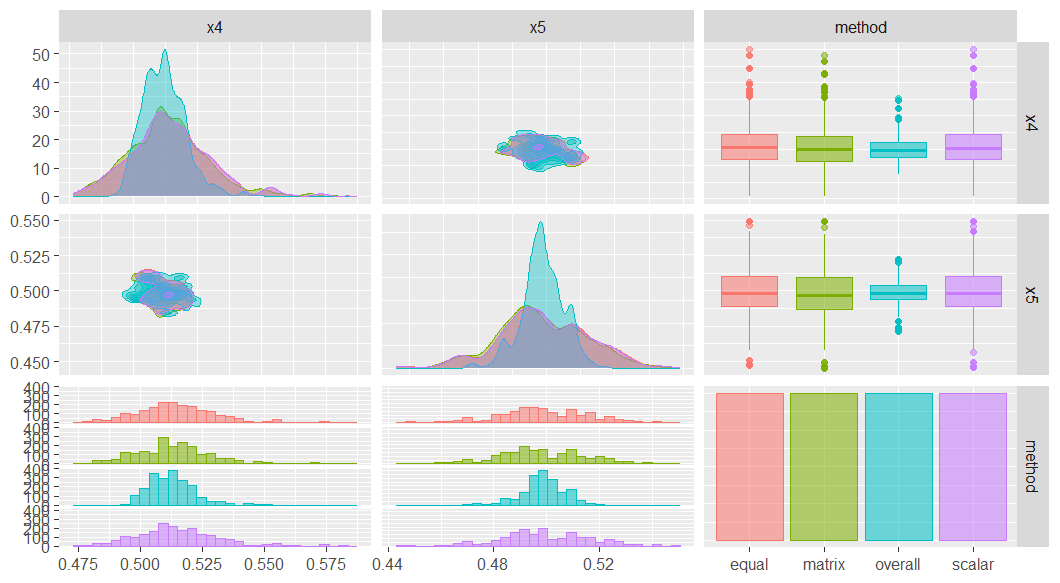
\includegraphics[width=340pt, height=200pt]{Chapters/chapter13/figures/CMC.png}
	\caption{Simulation: Posterior distributions from consensus Monte Carlo in logit simulation exercise}
	\label{CMCogit}
\end{figure} 


To implement the SGLD algorithm (Algorithm~\ref{Alg:SGLD}), we set \( n = 0.01 \cdot N \), and the step size to \( 1 \times 10^{-4} \). The following code illustrates how to implement the SGLD algorithm.\footnote{There is an \textbf{R} package called \textit{sgmcmc}, developed by \cite{baker2019sgmcmc}, which provides implementations of various stochastic gradient MCMC methods, including SGLD and SGHMC. However, this package depends on version~1 of the \textit{tensorflow} package, while the current version is 2, and \textit{sgmcmc} has not been updated on CRAN. We attempted to install the package from its GitHub repository using the \texttt{devtools::install\_github("STOR-i/sgmcmc")} command, but encountered compatibility issues due to conflicting TensorFlow versions.} 

In Exercise~8, you are asked to implement the control variate version of SGLD. Begin by running 1{,}500 SGD iterations to locate the posterior mode. This mode should then be used as the initial value for a subsequent run of 1{,}000 SGLD iterations.

By running the code, you can verify that the computational time of the SGLD algorithm is lower than that of the Metropolis–Hastings algorithm. Figure~\ref{SGLDlogit} shows the posterior distributions of the fifth location parameter obtained from SGLD and Metropolis–Hastings. We observe that both modes are centered around the true population value; however, the SGLD distribution exhibits greater dispersion compared to the Metropolis–Hastings distribution.


\begin{tcolorbox}[enhanced,width=4.67in,center upper,
	fontupper=\large\bfseries,drop shadow southwest,sharp corners]
	\textit{R code. Stochastic Gradient Langevin Dynamic (SGLD): Logit regression}
	\begin{VF}
		\begin{lstlisting}[language=R]
SGLD_step <- function(beta, y, X, stepsize, batch_size, prior_var = 10) {
	N <- nrow(X); 	K <- length(beta)
	ids <- sample(1:N, size = batch_size, replace = FALSE)
	grad <- rep(0, K)
	for (i in ids) {
		xi <- X[i, ]
		eta <- sum(xi * beta)
		pi <- 1 / (1 + exp(-eta))
		grad_i <- -(y[i] - pi) * xi
		grad <- grad + grad_i
	}
	grad <- grad / batch_size * N
	grad <- grad + beta / prior_var  # gradient of log-prior
	noise <- rnorm(K, 0, sqrt(stepsize))
	beta_new <- beta - 0.5 * stepsize * grad + noise
	return(beta_new)
}
#--- SGLD algorithm
run_SGLD <- function(y, X, stepsize, batch_prop, n_iter, burnin, beta_init = NULL) {
	N <- nrow(X)
	K <- ncol(X)
	batch_size <- round(batch_prop * N)
	
	beta_mat <- matrix(0, n_iter + burnin, K)
	beta_mat[1, ] <- if (is.null(beta_init)) rep(0, K) else beta_init
	
	for (s in 2:(n_iter + burnin)) {
		beta_mat[s, ] <- SGLD_step(beta_mat[s - 1, ], y, X, stepsize, batch_size)
	}
	beta_mat[(burnin + 1):(n_iter + burnin), ]
}
#--- Run SGLD
posterior_sgld <- run_SGLD(y = y, X = X, stepsize, batch_prop, n_iter, burnin)
#--- Compare densities for beta5
df_plot <- data.frame(
value = c(posterior_sgld[, k_target2], posterior_mh[, k_target2]),
method = rep(c("SGLD", "MCMC"), each = n_iter)
)
ggplot(df_plot, aes(x = value, fill = method, color = method)) + geom_density(alpha = 0.4) + geom_vline(xintercept = beta_true[k_target2], linetype = "dashed", color = "black") + labs(title = expression(paste("Posterior density of ", beta[5])), x = expression(beta[5]), y = "Density") + theme_minimal()
\end{lstlisting}
	\end{VF}
\end{tcolorbox}

\begin{figure}[!h]
	\centering
	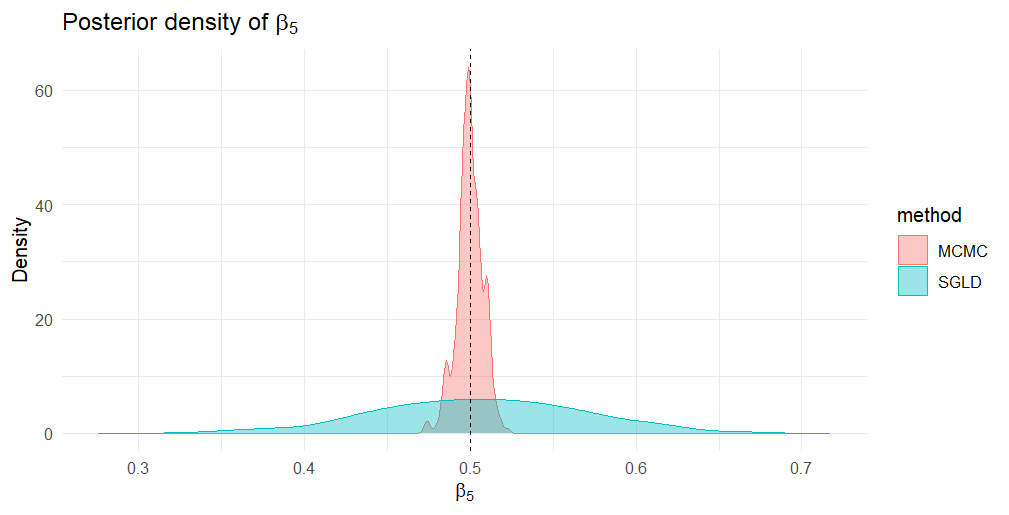
\includegraphics[width=340pt, height=200pt]{Chapters/chapter13/figures/SGLDlogit.png}
	\caption{Simulation: Posterior distributions from stochastic gradient Langevin Dynamic logit simulation exercise}
	\label{SGLDlogit}
\end{figure}  

\section{Summary}\label{13_6}

In this chapter, we introduced several Bayesian machine learning methods designed to address the challenges posed by \textit{wide} and \textit{tall} data. However, the field of Bayesian machine learning is rapidly evolving, and the material presented here should be viewed as an introductory overview. Many important topics were not covered but are highly relevant, such as Bayesian neural networks \cite{neal2012bayesian} and neural posterior estimation \cite{papamakarios2016fast,lueckmann2017flexible,greenberg2019automatic}. Other key approaches, such as Variational Bayes, particularly in its stochastic implementations, which are rooted in machine learning and offer scalable solutions for tall data, are introduced in Chapter~\ref{chap15} \cite{wainwright2008graphical}.

\section{Exercises}\label{13_7}

\begin{enumerate}
	\item \textbf{Simulation exercise: the Bayesian LASSO continues}
	
	Program the Gibbs sampler for the Bayesian LASSO from scratch, assuming a hierarchical structure for the global shrinkage parameter, where both the shape and rate parameters are set to 1. Perform inference using this sampler in the Bayesian LASSO simulation exercise and compare the results with those obtained using the \textit{monomvn} package.
	
	\item \cite{jetter2022postcold} employ SSVS to identify the main drivers of civil conflict in the post-Cold War era, considering a set of 35 potential determinants across 175 countries worldwide. We use a subset of their dataset provided in \textit{Conflict.csv}, where the dependent variable is \textit{conflictcw}, a binary indicator of civil conflict. Perform SSVS using the \textit{BoomSpikeSlab} package, specifically the \textit{lm.spike} function, to identify the best subset of models.
	
	\item \cite{tuchler2008bayesian} proposes an SSVS approach for binary response models. Use the dataset \textit{Conflict.csv}, where the dependent variable is \textit{conflictcw}, to perform SSVS using the \textit{BoomSpikeSlab} package, specifically the \textit{logit.spike} function, in order to identify the best subset of models. Compare the results with those obtained in Exercise 2.
	
	\item \textbf{Example: Simulation exercise $K > N$}
	
	Use the simulation setting from the Bayesian LASSO and SSVS examples, but now assume there are 600 inputs. This setup implies that the number of inputs exceeds the sample size. In such a scenario, there is no unique solution to the least squares estimator because the determinant of $\mathbf{W}^{\top} \mathbf{W}$ is zero. This means the matrix is not invertible, and consequently, standard inference procedures based on the least squares estimator cannot be applied. On the other hand, Bayesian inference in this setup is well-defined because the prior helps regularize the problem, which is a key motivation for these methods.
	
	\item \textbf{Simulation exercise: the BART model continues} 
	
	Compute Friedman’s partial dependence functions \cite{friedman2001greedy} for all variables in the BART model simulation example, and plot the posterior mean along with the 95\% credible intervals.
	
	\item \cite{chipman2010bart} presents BART probit for classification. This method can be implemented using the \textit{BART} package through the function \textit{pbart}. Use the file \textit{Conflict.csv}, where the dependent variable is \textit{conflictcw}, to perform BART probit, implementing \textit{k-fold} cross-validation to select the threshold that maximizes the sum of the true positive and true negative rates. Additionally, identify the most important predictors by evaluating different numbers of trees.
	
	
	\item \textbf{Simulation exercise: The Gaussian Process simulation continues}
	
	Simulate the process
	\[
	f_i = \sin(2\pi x_{i1}) + \cos(2\pi x_{i2}) + \sin(x_{i1} x_{i2}) + \mu_i,
	\]
	where \( \mu_i \overset{\text{i.i.d.}}{\sim} {N}(0, 0.1^2) \), \( x_{ik} \sim {U}(0,1) \) for \( k = 1, 2 \), and the sample size is 500. 
	
	Define a grid of 20 evenly spaced values between 0 and 1 for each covariate \( x_{ik} \), and use this grid to perform prediction.
	
	Estimate the hyperparameters of the Gaussian Process by maximizing the log marginal likelihood. Then, use the \textit{km} function from the \textit{DiceKriging} package to fit the Gaussian Process, fixing the noise variance at the value that maximizes the log marginal likelihood.
	
	Finally, use the fitted model to predict the outputs on the grid points, and produce a 3D plot showing the predicted surface along with the training data points.
	
	\item \textbf{Simulation exercise: Stochastic gradient MCMC continues} 
	
	Program from scratch the stochastic gradient Langevin dynamic algorithm for the logit simulation exercise implementing the control variate version performing 1{,}500 stochastic gradient descent iterations to locate the posterior mode, which should be then used as the initial value for 1{,}000 subsequent MCMC iterations using a step size set to \(1 \times 10^{-4}\).
	
	\item Perform the simulation according to the model \( y_i = 1 - 2 x_{i1} + 0.5 x_{i2} + \mu_i \), where \( \mu_i \sim {N}(0,1) \), the sample size is 100{,}000, and the covariates \( \mathbf{x}_i \sim {N}(\mathbf{0}, \mathbf{I}_2) \). Use 5{,}000 MCMC iterations and a batch size of 1{,}000 to implement the SGLD algorithm. Set a learning rate schedule that yields sensible results.
	
	Assume independent priors \( \pi(\boldsymbol{\beta}, \sigma^2) = \pi(\boldsymbol{\beta}) \times \pi(\sigma^2) \), with \( \boldsymbol{\beta} \sim {N}(\mathbf{0}, \mathbf{I}_3) \) and \( \sigma^2 \sim {IG}(\alpha_0/2, \delta_0/2) \), where \( \alpha_0 = \delta_0 = 0.01 \).
	
	
	  
\end{enumerate}

